\documentclass[12pt, a4paper]{article}
%=========================== PACKAGES =============================%

\usepackage[utf8]{inputenc}
\DeclareUnicodeCharacter{00A0}{ }

\usepackage[hmargin=1.5cm,vmargin=1.5cm]{geometry}
\usepackage[brazil]{babel}

\usepackage{longtable}

\usepackage{graphicx}
\usepackage{placeins}
\usepackage{subcaption}
\usepackage{float}

\usepackage{hhline}
\usepackage{courier}
 
\usepackage{amsmath}
\usepackage{bm}
\usepackage{amsfonts}

\usepackage{hyperref}

\usepackage{listings}
\renewcommand\lstlistingname{Programa}
 

\usepackage{color} %red, green, blue, yellow, cyan, magenta, black, white
\definecolor{mygreen}{RGB}{28,140,0} % color values Red, Green, Blue
\definecolor{mylilas}{RGB}{170,55,241} 
\lstset{language=Matlab,%
    %basicstyle=\color{red},
    basicstyle=\footnotesize\ttfamily,
    breaklines=true,%
    morekeywords={matlab2tikz},
%    keywordstyle=\color{blue},%
    morekeywords=[2]{1}, keywordstyle=[2]{\color{black}},
%    identifierstyle=\color{black},%
%    stringstyle=\color{mylilas},
%    commentstyle=\color{mygreen},%
    showstringspaces=false,%without this there will be a symbol in the places where there is a space
    numbers=left,%
    numberstyle={\tiny \color{black}},% size of the numbers
    numbersep=9pt, % this defines how far the numbers are from the text
    %emph=[1]{for,end,break},emphstyle=[1]\color{red}, %some words to emphasise
    %emph=[2]{word1,word2}, emphstyle=[2]{style},    
    frame= single,
}
 
\lstdefinestyle{nonumbers}
{numbers=none}

\usepackage{multirow}


\usepackage{steinmetz}
\usepackage{float}

%=========================== PACKAGES =============================%


\author{Gustavo Ciotto Pinton}

\begin{document}

\begin{titlepage}
\vspace*{.28\textheight}
\begin{center}
%
\begin{figure}[h]
    \centering
    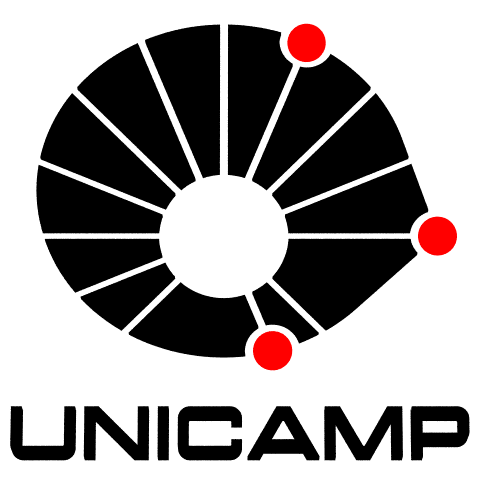
\includegraphics[scale=0.18]{image/LogoUnicamp}
\end{figure} 
%
\vspace*{10pt}
%\text{ }\\[7 cm]
\textbf{\LARGE Exercício de Fixação de Conceitos 2} \\ \vspace{12pt}
\textbf{\large EA072 - Inteligência Artificial em Aplicações Industriais}
\vspace*{72pt}

Gustavo \textbf{CIOTTO PINTON} - \textbf{RA 117136}
 

Campinas, \today

\end{center}
\end{titlepage}

\newpage
%  
% {\large 
%     \centerline{\textbf{Exercício de Fixação de Conceitos 1}}
%     \centerline{Gustavo Ciotto Pinton - 117136}
%     \centerline{EA072 - Inteligência Artificial em Aplicações Industriais}
% }

\section{Síntese de controle PID}
\label{sec:pid}
 
\begin {enumerate}
  \item Antes de definirmos os operadores de mutação e \textit{crossover}, é
  necessário diferenciarmos estes dois conceitos. Embora ambos ocorram em
  organismos biológicos e sejam responsáveis pela alteração do genótipo de um
  indivíduo, estes mecanismos ocorrem em diferentes etapas da vida do respectivo
  organismo. O termo \textit{mutação} é utilizado para descrever o processo no
  qual um alelo de um gene é \textbf{aleatoriamente} substituído ou modificado
  por outro. Em termos matemáticos, sejam os índices \(r, \ldots, u\) as
  posições que sofrerão mutação e que foram determinadas aleatoriamente. Cada
  posição possui um probabalidade \(p_m\) de ser submetida a este processo. Ao
  final da mutação, os alelos referentes a estes índices serão modificados, no
  caso de uma codificação em ponto flutuante, segundo uma distribuição
  \textit{uniforme} ou \textit{não uniforme}. No caso da \textit{não uniforme},
  insere-se uma perturbação com distribuição \textit{normal} com média nula na
  posição escolhida e desvio-padrão decrescente ao longo das gerações, o que
  garante consequentemente um refinamento da solução à medida que nos
  aproximamos de resultados ótimos. 
  
  O processo de \textit{crossover}, por sua vez, trata-se de um mecanismo de
  recombinação genética de dois ou mais cromossomos. Para a codificação de
  algoritmos evolutivos em que os cromossomos possuem valores em ponto
  flutuante, destacam-se duas técnicas: o \textit{crossover} aritmético e o
  uniforme. Para o primeiro, a partir dos cromossomos \(\textbf{x}\) e \(\textbf{y}\),
  obtém-se uma combinção convexa dos valores dos genes de \(\textbf{x}\) e
  \(\textbf{y}\), isto é, o cromossomo \(a\textbf{x} + (1-a)\textbf{y}\), em que
  \(a \in [0, +1]\). Para o segundo, os genes dos cromossomos pais são
  escolhidos com igual probabilidade para formar um cromossomo filho. Por
  exemplo, se a probabilidade vale 0.5, então espera-se que o cromossomo
  resultante seja composto por metade dos genes de \textbf{x} e metade de
  \textbf{y}.
  
  Outra etapa importante para os algoritmos evolutivos é a seleção dos
  indivíduos mais ``adaptados'' ao problema (que possuem maior função de
  \textit{fitness}). Este processo deve garantir que os melhores indivíduos
  persistam, mas não deve ser extremamente radical a fim de garantir uma
  diversidade na população. Um exemplo de um operador de seleção é a técnica de
  \textit{seleção por torneio}. Para selecionar \(N\) indivíduos, realizam-se
  \(N\) torneios com \(p\) participantes, escolhidos aleatoriamente. Quanto mais
  alto é \(p\), maior é a pressão seletiva, isto é, para um indivíduo ruim ser
  escolhido ao menos em um torneio, é necessário que ele compita com \(p-1\)
  indivíduos piores que ele (para \(p\) grande, a probabilidade deste fato
  ocorrer é muito pequena). Cada torneio é vencido pelo indivíduo que apresenta maior
  \textit{fitness}. No caso deste exercício, será realizado apenas um torneio,
  que é composto por 3 indivíduos.

  \item As constantes rrier 
    apresentadas na tabela \ref{tab:pid_constantes} a seguir
  foram definidas no arquivo \texttt{prog\_PID.m}, disponibilizado pelo
  professor.
  
  \begin{table}[h]
	    \centering
		\caption{\label{tab:pid_constantes} Constantes definidas em
		\texttt{prog\_PID.m}}
		\begin{tabular}{|c | c |}
			\hline
			\textbf{Atributos} & \textbf{Valor} \\	\hhline{|=|=|}
			Tamanho da População & 100 \\ \hline 
			Número máximo de Gerações & 50 \\ \hline 
			Taxa de Mutação & 0.4 \\ \hline 			
			Taxa de Crossover & 0.8 \\ \hline 			
		\end{tabular}	    
    \end{table} 
    
    Observa-se taxas de mutação e \textit{crossover} relativamente altas: para a
    primeira, um alelo tem probalidade de 40\% de ser mutado, isto é, ele possui
    aproximadamente a metade das chances de ser modificado. Em relação ao
    tamanho da população e o número de gerações , 100 e 50 são
    números suficientemente grandes para garantir, respectivamente,	 diversidade
    entre os indivíduos e uma boa qualidade no resultado visto a quantidade de
    recombinações entre os cromossomos que serão realizadas.
    
    A população inicial é obtida pelo comando \texttt{pop =
    5*rand(tam\_pop,3);}, em que \texttt{rand} é uma função do MATLAB que gera
    números aleatórios segundo uma distribuição uniforme e \texttt{tam\_pop}
    vale 100. Será criada, portanto, uma matriz de 100 linhas, cada uma
    representando um indivíduo, e 3 colunas, uma para cada constante a ser
    determinada \(k_p\), \(k_d\) e \(k_i\).
    
    Finalmente, cada operador de \textit{crossover} é escolhido com 50\% de
    probabilidade. Espera-se portanto que o operador aritmétido seja escolhido
    em metade das oportunidades e o uniforme, também.
    
    \item Após adicionarmos as linhas referentes ao cálculo do \textit{fitness},
    as execuções do programa \textit{prog\_pid.m} resultam nos dados da tabela
    \ref{tab:pid_c}.
    
    \begin{table}[h]
	    \centering
		\caption{\label{tab:pid_c} Resultados das 5 execuções de
		\texttt{prog\_PID.m}}
		\begin{tabular}{| c | c | c | c | c | c | c | c | c |}
			\hline
			\textbf{Ex.} & \(k_p\) & \(k_d\) & \(k_i\) &
			\(t_{subida} \) (s) & \(t_{estabilizacao}\) (s) & \textit{Overshoot} (\%) &
			\(\Delta \phi\) (º)& \textit{Fitness}\\ \hhline{|=|=|=|=|=|=|=|=|=|}
			1 & 4.9935 & 2.385e-05 & 4.46633 & 0.0064396 & 3.26286 &  97.7286  &
			1.1935 & 9.9360\\ \hline 
			2 & 4.9960 & 2.296e-05 & 3.99303 & 0.0064393 & 3.14669 & 97.6506 & 
			1.2340 & 9.9360 \\
			\hline 3 & 4.9923 & 1.350e-05 & 3.95399 & 0.0064397 & 3.3217 & 97.7735 &
			1.1687 & 9.9360	\\
			\hline 4 & 4.9940 & 2.240e-05 & 4.33452 & 0.0064395 & 3.24405 & 97.7234 &
			1.1960 & 9.9360\\
			\hline 5 & 4.9990 & 1.528e-05 & 4.4244 & 0.0064348 & 3.41617  & 97.8392 &
			1.1346 & 9.9361 \\ 
			\hline
		\end{tabular}	    
    \end{table}
    
    Observa-se que todos os valores \(k_d\) relativos à ação derivadora são
    praticamente nulos e que \(k_i\) e \(k_p\) encontram-se muito próximos a
    seus valores máximos, isto é, 5. Isto indica que a ação derivadora não
    exerce efeitos importantes sobre o tempo de resposta apresentado pelo
    sistema.    Os valores de tempo dos primeiros máximos em todas as execuções
    concentram-se em torno do valor \(t_{subida} = 0.00644\) s. Sabe-se também
    que este atributo é fortemente ligado à frequência de oscilação que a
    resposta ao degrau apresentará. Para sistemas de segunda ordem, por exemplo,
    a relação \(w_0t_m \approx 3\) evidencia o compromisso entre essas duas
    características.  Portanto, para valores muito pequenos de \(t_{subida}\),
    teremos frequências \(w_0\) elevadas e vice-versa. É justamente esse
    comportamento que é observado neste caso: pelo fato de que a função de
    \textit{fitness} só levar em conta o tempo de resposta, obtém-se respostas
    muito rápidas, porém que oscilam fortemente em torno de 1. A margem de fase
    (\(\Delta \phi\)) também possui uma relação com o \textit{overshoot}:
    pequenas margens de fase produzem sistemas menos estáveis e que apresentam
    maior erros percentuais entre a entrada e a saída. No nosso caso, como não
    nos preocupamos com esse parâmetro, obtém-se pequenas margens de fase e,
    consequentemente, grandes erros antes da estabilização. A figura
    \ref{fig:pid_step_c}, que é o resultado de uma das execuções acima, permite
    a visualização destes comportamentos. A figura \ref{fig:pid_mutacao_c}, por
    sua vez, mostra a quantidade de mutações realizadas pelo algoritmo evolutivo
    no decorrer no programa. Conforme explicado anteriormente, essa quantidade
    deve ser decrescente, visto que os melhores indíviduos devem ser mantidos
    nas gerações finais. As figuras \ref{fig:pid_fitness_c} e
    \ref{fig:pid_parametros_c} mostram, respectivamente, a evolução dos valores
    da função de \textit{fitness} e dos parâmetros \(k_p\), \(k_i\) e \(k_d\).
    Para o primeiro, observa-se que o melhor \textit{fitness} permanece sempre
    próximo de 10 e que o \textit{fitness} médio aproxima-se gradualmente a este
    valor, indicando que a população esta se ``especializando'' e adaptando no
    problema. Para segundo, verifica-se que \(k_d\) é praticamente nulo em todas
    as gerações, \(k_p\) se estabiliza a partir da geração 10 e \(k_i\) varia
    fortemente até a geração 40. Estes fatos nos dizem que o parâmetro que mais
    influencia o tempo do primeiro máximo é a ação integradora.

    \FloatBarrier
			    
	\begin{figure}[h!]
	
	\centering
	
		\begin{subfigure}{.5\textwidth}
		  \centering
		  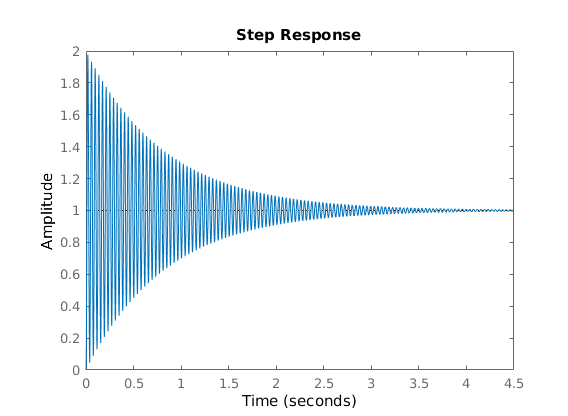
\includegraphics[width=1\linewidth]{pid/step_pid_ex_c}
		  \caption{Resposta ao degrau do sistema.}
		  \label{fig:pid_step_c}
		\end{subfigure}%
		\begin{subfigure}{.5\textwidth}
		  \centering
		  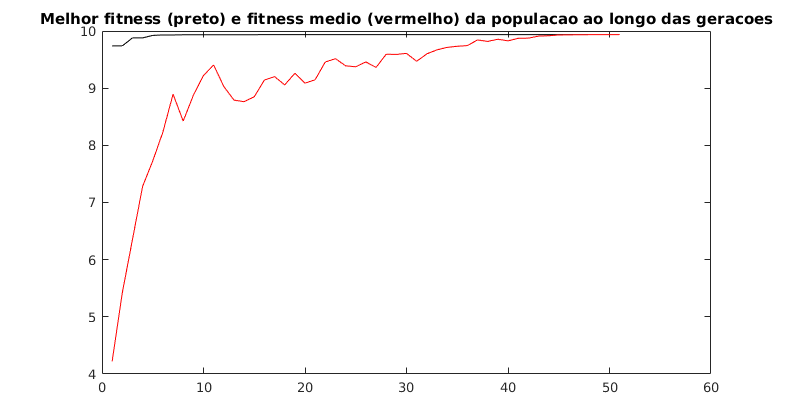
\includegraphics[width=1\linewidth]{pid/melhor_fitness_pid_ex_c}
		  \caption{Evolução dos valores da função \textit{fitness}.}
		  \label{fig:pid_fitness_c}
		\end{subfigure}%
		
		\begin{subfigure}{.5\textwidth}
		  \centering
		  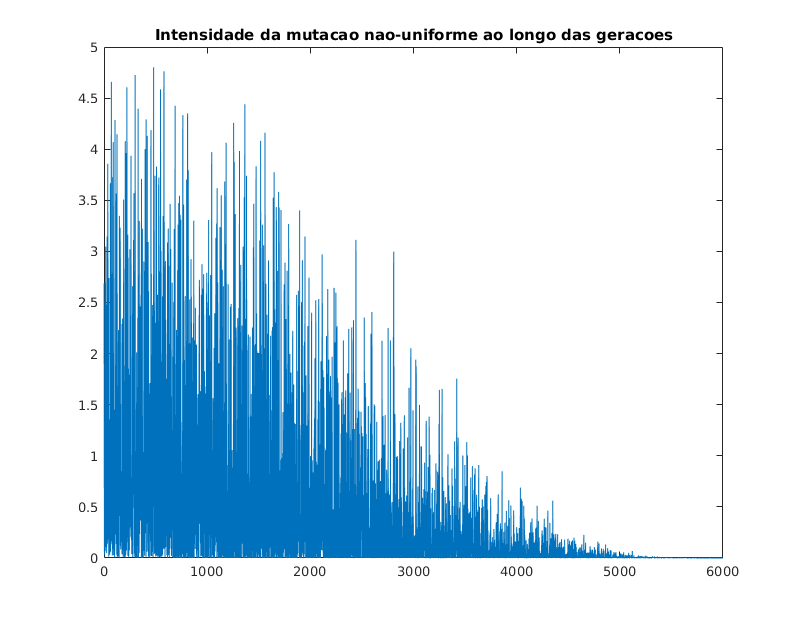
\includegraphics[width=1\linewidth]{pid/mutacao_pid_ex_c}
		  \caption{\centering Evolução da intensidade de mutações ao longo das
		  gerações.}
		  \label{fig:pid_mutacao_c}
		\end{subfigure}%
		\begin{subfigure}{.5\textwidth}
		  \centering
		  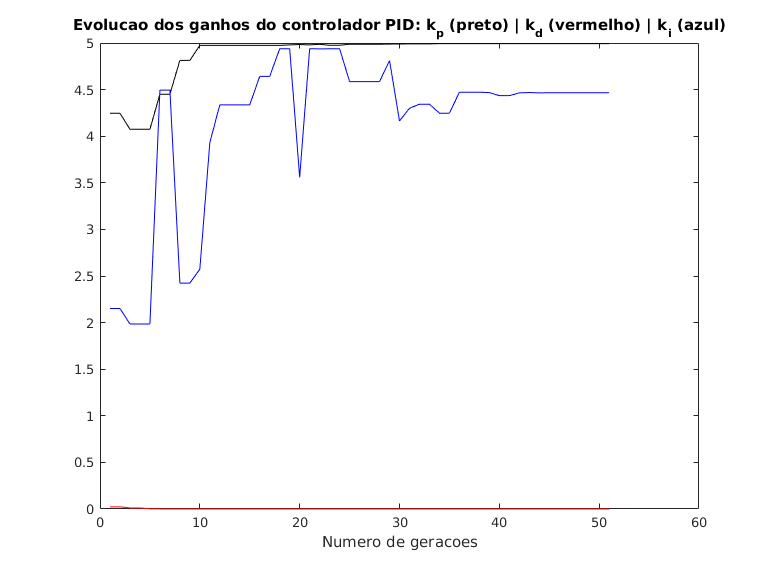
\includegraphics[width=1\linewidth]{pid/kp_kd_ki_pid_ex_c}
		  \caption{\centering Evolução dos parâmetros.}
		  \label{fig:pid_parametros_c} 
		\end{subfigure}
	
	\caption{Resultado para a execução 1 do algoritmo evolutivo.}
	\end{figure}
	
	
	\FloatBarrier
	
	 A modificação dos parâmetros da tabela \ref{tab:pid_constantes} pode
	 influenciar nos resultados acima. Se dobrarmos o número de indivíduos na
	 população, isto é, 200, e aumentarmos as taxas de crossover e mutação para,
	 respectivamente, 0.9 e 0.6, obtém-se os dados contidos na tabela
	 \ref{tab:pid_c_2}.
    
    \begin{table}[h]
	    \centering
		\caption{\label{tab:pid_c_2} Resultados da execução com os parâmetros
		modificados.}
		\begin{tabular}{| c | c | c | c | c | c | c | c |}
			\hline
			\(k_p\) & \(k_d\) & \(k_i\) &
			\(t_{subida} \) (s) & \(t_{estabilizacao}\) (s) & \textit{Overshoot} (\%) &
			\(\Delta \phi\) (º)& \textit{Fitness}\\ \hhline{|=|=|=|=|=|=|=|=|}
			4.9975 & 7.80994e-06 & 4.6839 & 0.00643281 & 3.68641 &  97.9919  &
			1.05405 & 9.93608\\ \hline 
		\end{tabular}	    
    \end{table}
    
    Observa-se que o tempo do primeiro máximo é ligeiramente inferior aos dos
    casos anteriores e, consequentemente, a função de \textit{fitness} é
    superior.  Os valores dos parâmetros continuam parecidos, sendo que \(k_d\)
    é inferior e \(k_i\) superior. De maneira geral, o aumento de recursos
    computacionais disponibilizados ao programa (aumento de população e
    quantidade de mutações) não causaram grandes diferenças nos resultados. As
    figuras \ref{fig:pid_fitness_c_mod} e \ref{fig:pid_parametros_c_mod}
    apresentam o mesmo comportamento descrito no parágrafo anterior e a
    \ref{fig:pid_mutacao_c_mod} destaca que a quantidade de mutações realizadas
    foi muito superior aos casos anteriores: observa-se que a presença de
    quantidades superiores a 10000 quando a taxa de mutação é 0.6.

	\FloatBarrier
			    
	\begin{figure}[h!]
	
	\centering
	
		\begin{subfigure}{.5\textwidth}
		  \centering
		  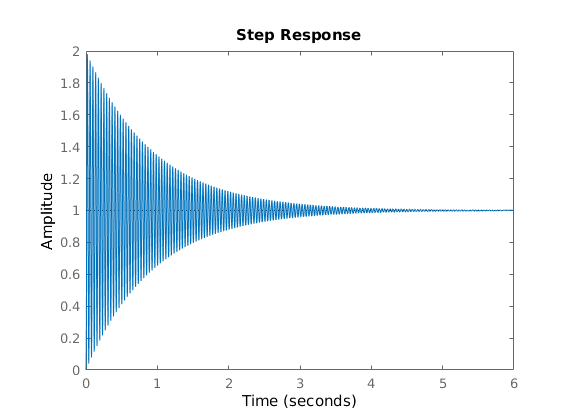
\includegraphics[width=1\linewidth]{pid/step_pid_ex_c_mod}
		  \caption{Resposta ao degrau do sistema.}
		  \label{fig:pid_step_c_mod}
		\end{subfigure}%
		\begin{subfigure}{.5\textwidth}
		  \centering
		  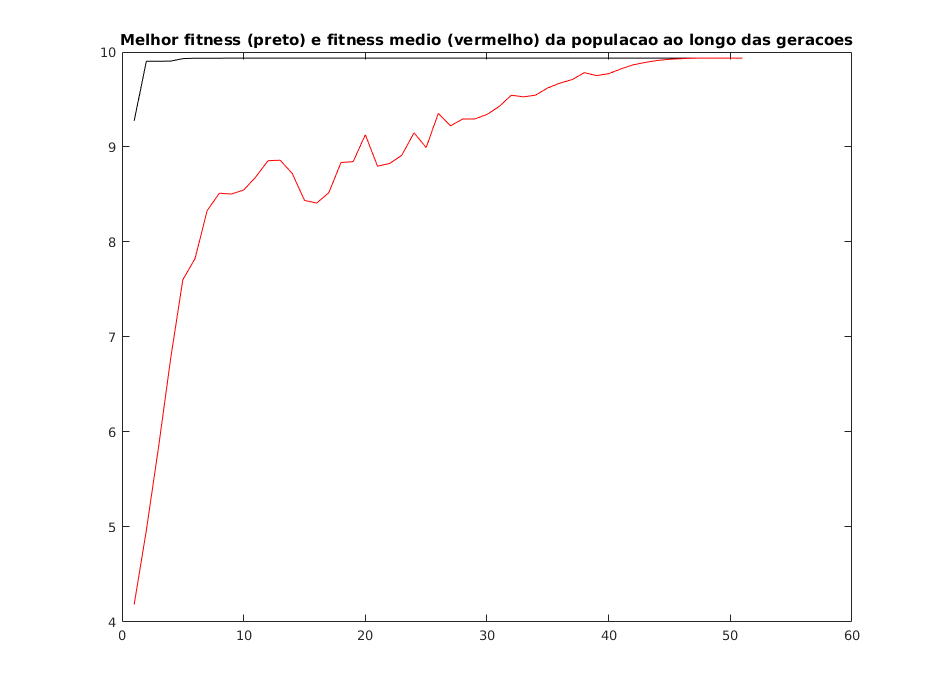
\includegraphics[width=1\linewidth]{pid/melhor_fitness_pid_ex_c_mod}
		  \caption{Evolução dos valores da função \textit{fitness}.}
		  \label{fig:pid_fitness_c_mod}
		\end{subfigure}%
		
		\begin{subfigure}{.5\textwidth}
		  \centering
		  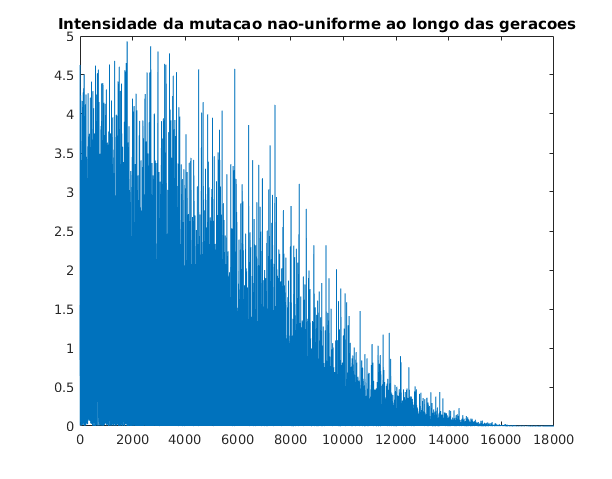
\includegraphics[width=1\linewidth]{pid/mutacao_pid_ex_c_mod}
		  \caption{\centering Evolução da intensidade de mutações ao longo das
		  gerações.}
		  \label{fig:pid_mutacao_c_mod}
		\end{subfigure}%
		\begin{subfigure}{.5\textwidth}
		  \centering
		  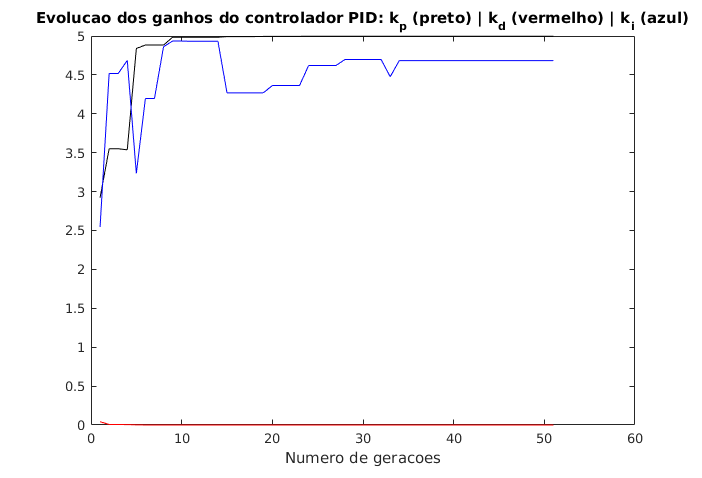
\includegraphics[width=1\linewidth]{pid/kp_kd_ki_pid_ex_c_mod}
		  \caption{\centering Evolução dos parâmetros.}
		  \label{fig:pid_parametros_c_mod} 
		\end{subfigure}
	
	\caption{Resultado para a execução do algoritmo evolutivo com parâmetros
	modificados.}
	\end{figure}

	\FloatBarrier
	
	\item Os resultados das 5 execuções com a nova função de \textit{fitness} estão
	presentes na tabela \ref{tab:pid_d}, logo abaixo. Dessa vez, considera-se
	também a margem de fase.
	
	\FloatBarrier
	
	\begin{table}[h]
	    \centering
		\caption{\label{tab:pid_d} Resultados das 5 execuções de
		\texttt{prog\_PID.m}}
		\vspace{-12pt}	
		\begin{tabular}{| c | c | c | c | c | c | c | c | c |}
			\hline
			\textbf{Ex.} & \(k_p\) & \(k_d\) & \(k_i\) &
			\(t_{subida} \) (s) & \(t_{estabilizacao}\) (s) & \textit{Overshoot} (\%) &
			\(\Delta \phi\) (º)& \textit{Fitness}\\ \hhline{|=|=|=|=|=|=|=|=|=|}
			1 & 1.22881 & 0.718353 & 4.54691 & 0.705398 & 12.7319 &  56.4502  &
			59.9346 & 5.53763\\ \hline 
			2 & 1.15518 & 0.57906 & 4.97227 & 0.605573 & 10.924 & 56.4079  & 
			59.9872 & 5.86308 \\
			\hline 3 & 0.812793 & 0.298811 & 4.76622 & 0.44429  & 8.01846 & 56.4355 &
			59.9522 & 6.47451	\\
			\hline 4 & 1.67979 & 1.23205 & 4.94384 & 0.885861 & 15.9772 & 56.398  &
			56.398  & 5.0356 \\
			\hline 5 & 2.36522 & 0.00523679 & 1.84369 & 0.0124718 & 0.100391 & 30.9773 &
			59.986 & 8.98883 \\ 
			\hline
		\end{tabular}	    
    \end{table}
    
    \FloatBarrier
    
    Ao contrário do item anterior, verifica-se neste caso uma grande variação
    nos melhores resultados nas diferentes execuções. As soluções 1 e 2
    apresentam soluções muito parecidas em todos os aspectos. A solução 4 foi a
    pior a ser encontrada e possui o maior valor de \(k_d\) encontrado. Isso
    leva a crer que grandes valores deste parâmetro influenciam negativamente no
    resultado, principalmente em relação à margem de fase: a pior margem foi
    encontrada nesta execução. A solução 5 foi aquela que melhor encontrou um
    compromisso entre tempo do primeiro máximo e estabilidade e, portanto,
    possui o maior \textit{fitness}. Remarcamos que os tempos de subida e
    estabilização e o \textit{overshoot} desta resposta foram muito inferiores a
    aqueles encontrados nas outras execuções, confirmando ainda mais a qualidade
    desta solução. Novamente, nos deparamos com o fato de que o ajuste de \(k_d\) é o
    mais sensível: grandes valores deste parâmetro não levam a bons resultados.
    Observa-se ainda que os outros dois parâmetros, \(k_p\) e \(k_i\), também
    apresentam grandes variações em relação as outras execuções, sendo \(k_d\)
    muito superior e \(k_i\) inferior. As imagens a seguir contém os gráficos
    gerados para a melhor execução. 
    
    \FloatBarrier
			    
	\begin{figure}[h!]
	
	\centering
	
		\begin{subfigure}{.5\textwidth}
		  \centering
		  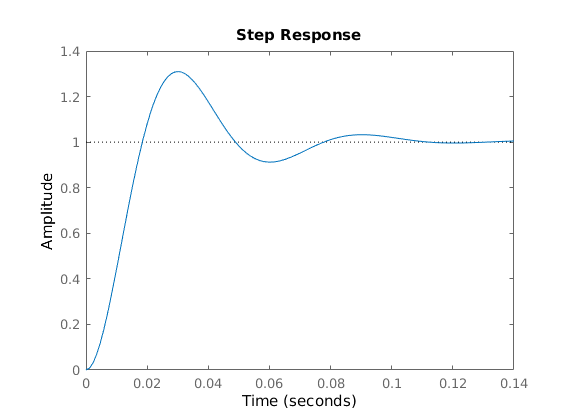
\includegraphics[width=1\linewidth]{pid/step_pid_ex_d_5}
		  \caption{Resposta ao degrau do sistema.}
		  \label{fig:pid_step_d_5}
		\end{subfigure}%
		\begin{subfigure}{.5\textwidth}
		  \centering
		  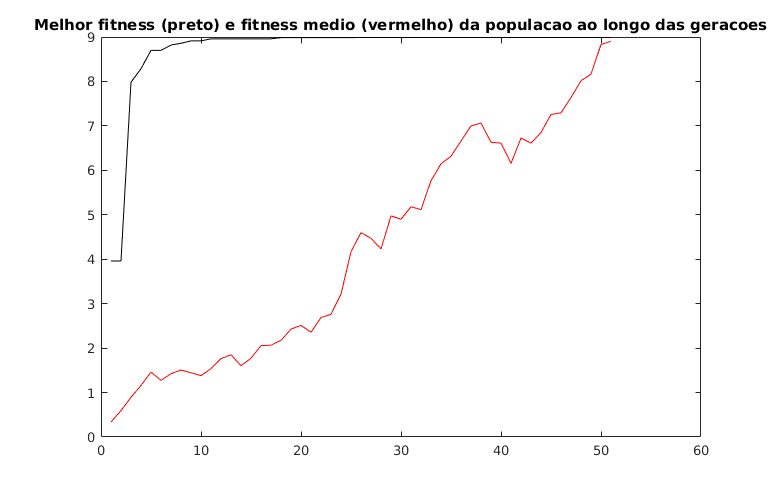
\includegraphics[width=1\linewidth]{pid/mutacao_pid_ex_d_5}
		  \caption{Evolução dos valores da função \textit{fitness}.}
		  \label{fig:pid_fitness_d_5}
		\end{subfigure}%
		
		\begin{subfigure}{.5\textwidth}
		  \centering
		  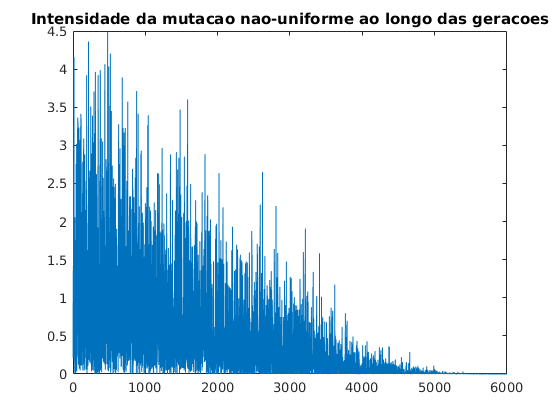
\includegraphics[width=1\linewidth]{pid/melhor_fitness_pid_ex_d_5}
		  \caption{\centering Evolução da intensidade de mutações ao longo das
		  gerações.}
		  \label{fig:pid_mutacao_d_5}
		\end{subfigure}%
		\begin{subfigure}{.5\textwidth}
		  \centering
		  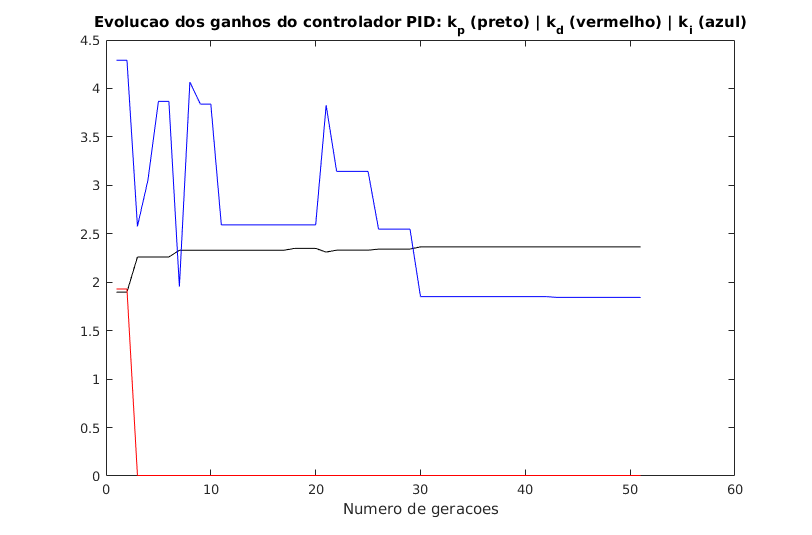
\includegraphics[width=1\linewidth]{pid/kp_kd_ki_pid_ex_d_5}
		  \caption{\centering Evolução dos parâmetros.}
		  \label{fig:pid_parametros_d_5} 
		\end{subfigure}
	
	\caption{Resultado para a melhor execução do algoritmo evolutivo com
	\textit{fitness} considerando a margem de fase.}
	\end{figure}
	
	\FloatBarrier
	
	A figura \ref{fig:pid_step_d_5} representa a resposta ao degrau do sistema com
	os parâmetros determinados na execução 5, cujas características já foram
	discutidas no parágrafo anterior. Na imagem \ref{fig:pid_fitness_d_5}, que
	apresenta a evolução do \textit{fitness}, observa-se que o melhor valor já é
	encontrado nas primeiras gerações. Entretanto, a quantia média ainda é muito
	inferior a tal valor, o que implica que a população é muito diversificada até a
	geração 50, isto é, poucos indivíduos se ``adaptaram'' tão bem quanto o
	melhor. A figura \ref{fig:pid_parametros_d_5} revela que o parâmetro que mais
	variou entre as gerações foi \(k_p\), assim como no caso do item anterior.
	
	\vspace{12pt}
	
	Os resultados obtidos com a função \textit{fitness} considerando
	o tempo de subida e também a margem de fase foram muito superiores em muitos
	aspectos:
	
	\begin{itemize}
		\item os valores de \textit{overshoot} no caso anterior eram, em média,
		de 97\%, sendo que neste item, encontra-se 30\%;
		
		\item a margem de fase no item anterior (\(\approx 2º\)) era muito inferior ao
		caso atual, em que exige-se \(\Delta \phi = 60º\), comprometendo fortemente a
		estabilidade do sistema;
	
		\item o tempo de subida no caso anterior era muito inferior ao atual, porém sua
		frequência de oscilação em torno de 1 era inaceitável;
	 
		\item no caso anterior, a resposta demorava muito a se estabilizar, o que pode
		representar um problema para algumas aplicações. No caso atual, encontra-se
		tempos de estabilização na ordem de centésimos de segundo;
	
	\end{itemize} 
	
	Enfim, efetuando as mesmas modificações realizadas anteriormente no tamanho da
	população e nas taxas de crossover e mutação, encontra-se os dados da tabela
	\ref{tab:pid_d_mod} e a imagems a seguir:
	
	\begin{table}[h]
	    \centering
		\caption{\label{tab:pid_d_mod} Resultados da execução com os parâmetros
		modificados.}
		\begin{tabular}{| c | c | c | c | c | c | c | c |} 
			\hline
			\(k_p\) & \(k_d\) & \(k_i\) &
			\(t_{subida} \) (s) & \(t_{estabilizacao}\) (s) & \textit{Overshoot} (\%) &
			\(\Delta \phi\) (º)& \textit{Fitness}\\ \hhline{|=|=|=|=|=|=|=|=|}
			2.57579 & 0.005528 & 3.77055 & 0.011941 & 0.09798 &  31.3347  &
			60.015 & 8.99308\\ \hline 
		\end{tabular}	    
    \end{table}
	
	\FloatBarrier
			    
	\begin{figure}[h!]
	
	\centering
	
		\begin{subfigure}{.5\textwidth}
		  \centering
		  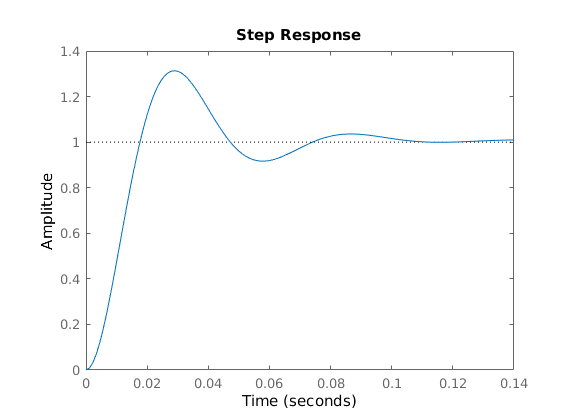
\includegraphics[width=1\linewidth]{pid/step_pid_ex_d_mod}
		  \caption{Resposta ao degrau do sistema.}
		  \label{fig:pid_step_d_mod}
		\end{subfigure}%
		\begin{subfigure}{.5\textwidth}
		  \centering
		  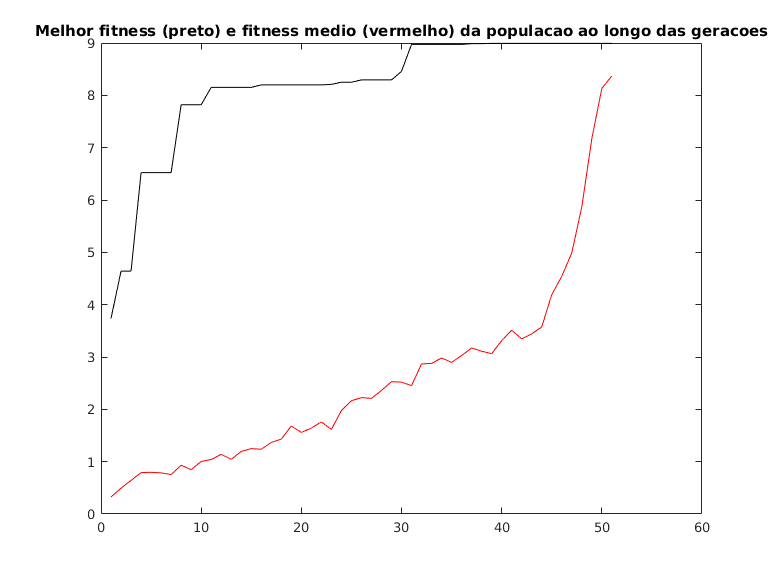
\includegraphics[width=1\linewidth]{pid/melhor_fitness_pid_ex_d_mod}
		  \caption{Evolução dos valores da função \textit{fitness}.}
		  \label{fig:pid_fitness_d_mod}
		\end{subfigure}%
		
		\begin{subfigure}{.5\textwidth}
		  \centering
		  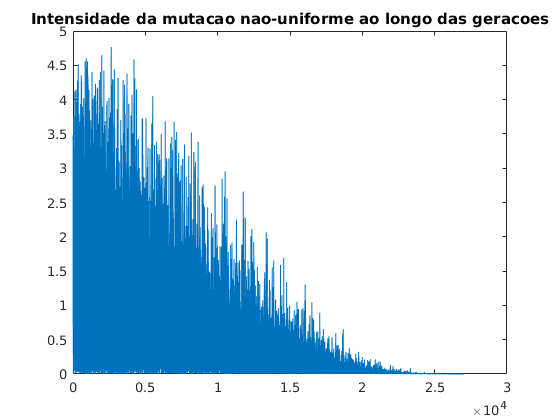
\includegraphics[width=1\linewidth]{pid/mutacao_pid_ex_d_mod}
		  \caption{\centering Evolução da intensidade de mutações ao longo das
		  gerações.}
		  \label{fig:pid_mutacao_d_5}
		\end{subfigure}%
		\begin{subfigure}{.5\textwidth}
		  \centering
		  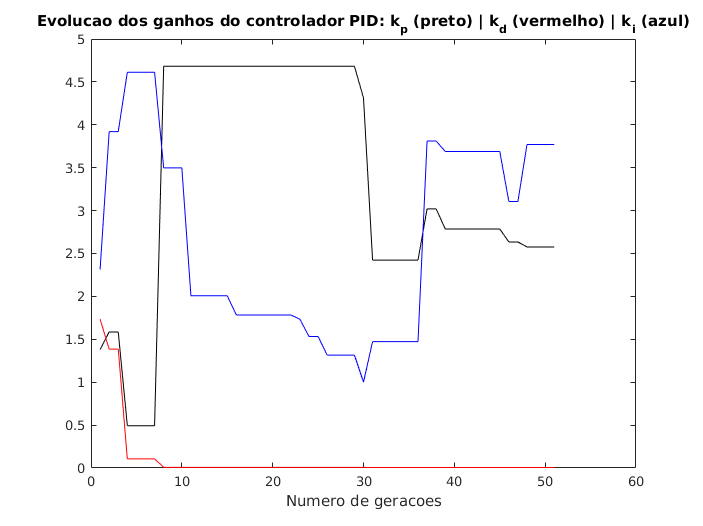
\includegraphics[width=1\linewidth]{pid/kp_kd_ki_pid_ex_d_mod}
		  \caption{\centering Evolução dos parâmetros.}
		  \label{fig:pid_parametros_d_mod} 
		\end{subfigure}
	
	\caption{Resultado para a melhor execução do algoritmo evolutivo com
	\textit{fitness} considerando a margem de fase e parâmetros modificados.}
	\end{figure}
	
	\FloatBarrier
	
	Neste caso, como os resultados de cada execução variam bastante, aumentar a
	população e as taxas de \textit{crossover} e mutação contribuem para a obtenção
	de uma solução de melhor qualidade, visto que a diversidade nos indivíduos é
	maior. Logo, a probabilidade que a solução ótima esteja presente em um dos
	indivíduos é consequentemente maior. Uma taxa de mutação elevada também garante
	que mais soluções sejam testadas, à medida que bons indivíduos podem dar origem
	a indivíduos melhores que eles mesmos através da mutação. Enfim, assim como no
	caso em que os parâmetros não tinham sido alterados, a figura
	\ref{fig:pid_fitness_d_mod} revela que a média dos valores de \textit{fitness}
	é muito distante do maior, indicando que nas gerações mais jovens há muitos
	indivíduos ruins. A figura \ref{fig:pid_parametros_d_mod} mostra, por sua vez,
	que, para populações maiores, todos os parâmetros podem variar fortemente
	ao passar das gerações, ao contrário que é observado no caso em que tamanho da
	população é igual a 100. Este fato também é totalmente esperado, visto que,
	para populações maiores, a chance de um indivíduo encontrar um outro melhor que ele
	é maior.
	
\end{enumerate}

\section{Aproximação de funções multidimensionais}

\subsection {Mapeamento y = f(x)}

A função escolhida para o mapeamento \(\mathbb{R}^1 \rightarrow \mathbb{R}^1\)
está representada logo abaixo. Foi definido que o intervalo de \(x\) é
\([-2\pi,2\pi]\) e que este intervalo seria discretizado a cada 0.01, a fim de
possuirmos uma quantidade grande de amostras, isto é, 1257.

\begin{equation}
y = \exp(\sin x + \cos x) + \left|x\right|
\label{eq:map1}
\end{equation}

Sem a presença de ruídos, este mapeamento produz a imagem
\ref{fig:map1_s_ruido}. A imagem \ref{fig:map1_c_ruido}, por sua vez, apresenta
o resultado da soma da função com um ruído de distribuição normal de média nula
e variância 0.64. É possível verificar que a adição do ruído prejudica
fortemente a identificação do formato inicial do mapeamento. 

\FloatBarrier
			    
	\begin{figure}[h!]
	
	\centering
	
		\begin{subfigure}{.5\textwidth} 
		  \centering
		  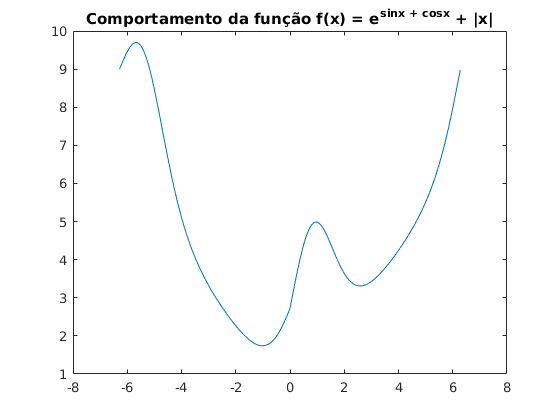
\includegraphics[width=1\linewidth]{image/sem_ruidos_y_fx}
		  \caption{\centering Mapeamento sem ruídos.} 
		  \label{fig:map1_s_ruido} 
		  
		\end{subfigure}%
		\begin{subfigure}{.5\textwidth}
		  \centering
		  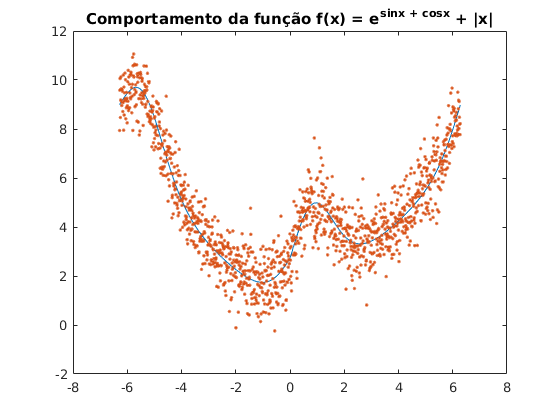
\includegraphics[width=1\linewidth]{image/com_ruidos_y_fx}
		  \caption{\centering Mapeamento com ruídos.}
		  \label{fig:map1_c_ruido} 
		\end{subfigure}
	
	
	\caption{Mapeamento da função \ref{eq:map1}.}
	\end{figure}
	
	\FloatBarrier
	
A simulação realizada no \textit{Eureqa}, primeiramente com os dados sem ruídos
e habilitando-se as funções-base exp(), sin(), cos(), abs() e as operações
básicas, forneceu os resultados contidos nas figuras
\ref{fig:map1_solucoes_s_ruido} e \ref{fig:map1_pareto_s_ruido}. A primeira
lista as soluções encontradas que mais se aproximaram dos dados amostrais.
Destaca-se que a primeira solução, cujo peso é 40, é justamente aquela que
utilizamos para produzir os dados. A segunda imagem ilustra o compromisso entre
acurácia (erro) e simplicidade (complexidade da solução). Observa-se que
inúmeras soluções apresentam erro praticamente nulo, porém existe apenas uma
cuja complexidade é mínima para este caso. Essa função trata-se da solução de
tamanho 40 que, como já foi dito, é igual à equação \ref{eq:map1}. A figura
\ref{fig:map1_best_s_ruido} apresenta um resumo da melhor solução encontrada.
Destaca-se que o erro podem ser considerados como nulos, visto que o maior erro
encontrado foi da ordem de \(10^{-14}\).

\FloatBarrier
			    
	\begin{figure}[h!]
	
	\centering
	
		\begin{subfigure}{.45\textwidth} 
		  \centering
		  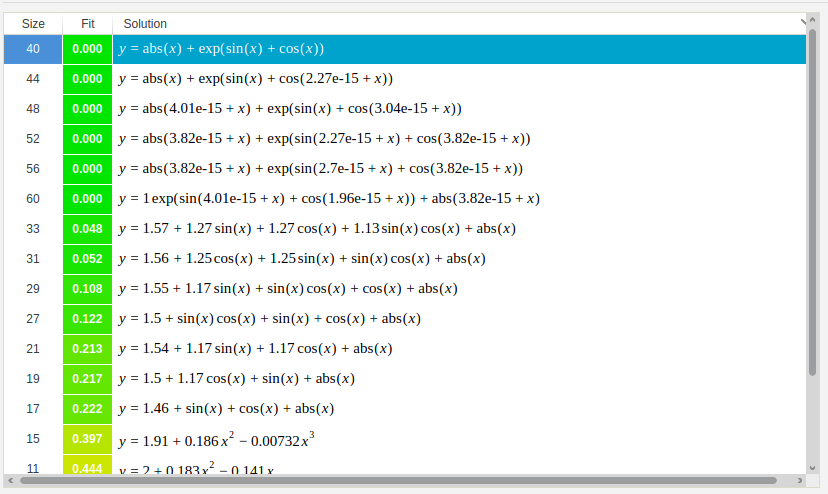
\includegraphics[width=1\linewidth]{image/solucoes_map1}
		  \caption{\centering Soluções encontradas pelo software.} 
		  \label{fig:map1_solucoes_s_ruido} 
		\end{subfigure}%
		\begin{subfigure}{.55\textwidth}
		  \centering
		  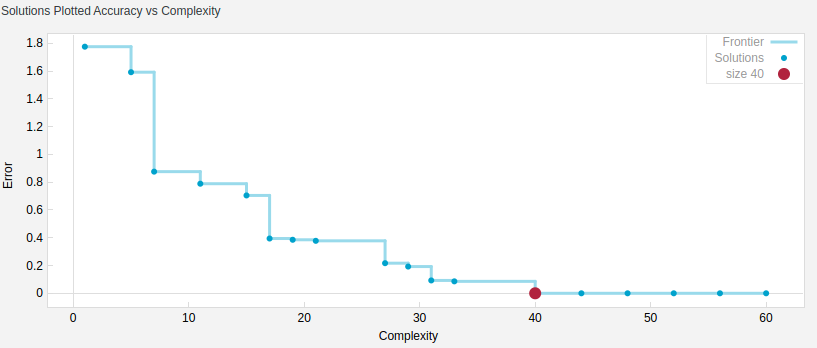
\includegraphics[width=1\linewidth]{image/pareto_map1}
		  \caption{\centering Compromisso acurácia \textit{x} simplicidade das
		  soluções.}
		  \label{fig:map1_pareto_s_ruido} 
		\end{subfigure}
	
		\begin{subfigure}{.65\textwidth}
		  \centering
		  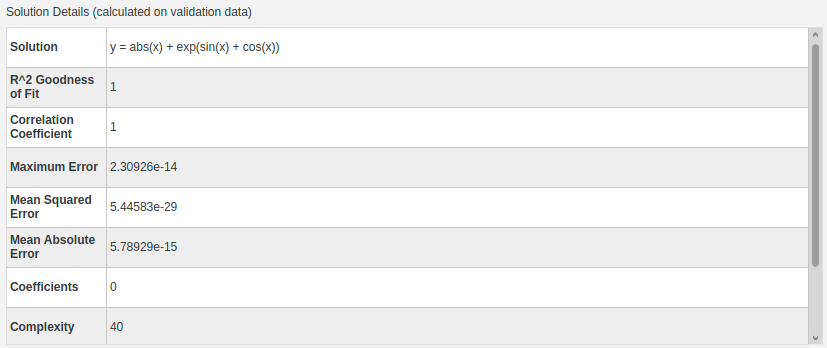
\includegraphics[width=1\linewidth]{image/best_solucao_map1}
		  \caption{\centering Resumo da melhor solução encontrada.}
		  \label{fig:map1_best_s_ruido} 
		\end{subfigure}
	
	\caption{Resultados para mapeamento da função \ref{eq:map1} sem ruídos.}
	\end{figure}
	
	\FloatBarrier

A simulação executada com os dados com ruído produziu o mapeamento representado
pela equação \ref{eq:map1_r}. A figura \ref{fig:comparaca_map1}  compara o mapeamento produzido
nesta fase com aquele utilizado para gerar os dados. Observa-se que ambos os
mapeamento estão muito próximos, porém há regiões em que as diferenças são
notáveis. Os resultados gerados pelo \textit{software} são, portanto, bastante
satisfatórios.

\begin{equation}
y = 1.61175 + 1.830094*\sin(0.792661 + x) +
0.55764*\sin(1.99325*x) + |x|
\label{eq:map1_r}
\end{equation}

\FloatBarrier
\begin{figure}[H]
		  \centering
		  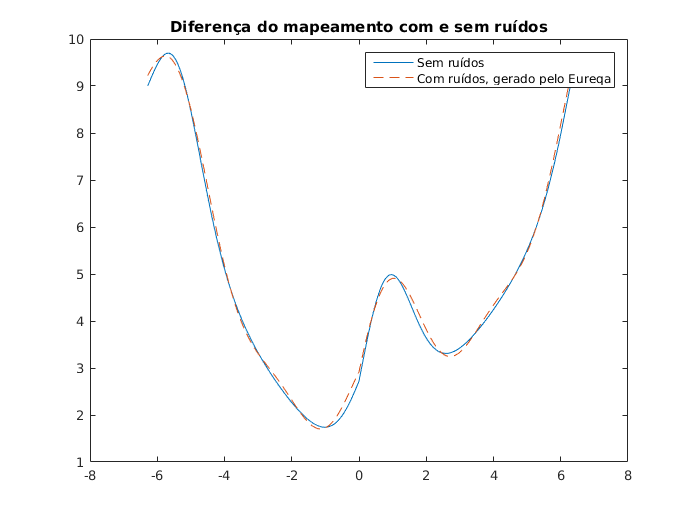
\includegraphics[width=0.65\linewidth]{image/comparacao_map1}
		  \caption{Comparação entre mapeamento com e sem ruídos.} 
		  \label{fig:comparaca_map1} 
		  
		\end{figure}
\FloatBarrier

As figuras \ref{fig:map1_solucoes_c_ruido}, \ref{fig:map1_pareto_c_ruido},
\ref{fig:map1_best_c_ruido}  e \ref{fig:map1_c_ruido} foram geradas pelo
\textit{Eureqa} e possuem informações sobre a solução encontrada. A primeira
é a lista de soluções encontradas pelo \textit{software}, a segunda mostra o
compromisso acurácia x complexidade (neste caso, a solução apresentada na
equação \ref{eq:map1_r} possui melhor compromisso, visto que seu erro é próximo
de 0 e sua complexidade, mínima), a terceira contem algumas informações sobre
a melhor solução (o erro quadrático médio neste caso é considerável,
contrariarmente ao caso sem ruído, e vale 0.625) e a última revela quais dados
foram usados para treinamento e validação, assim como o mapeamento encontrado.

\FloatBarrier
			    
	\begin{figure}[h!]
	
	\centering
	
		\begin{subfigure}{.45\textwidth} 
		  \centering
		  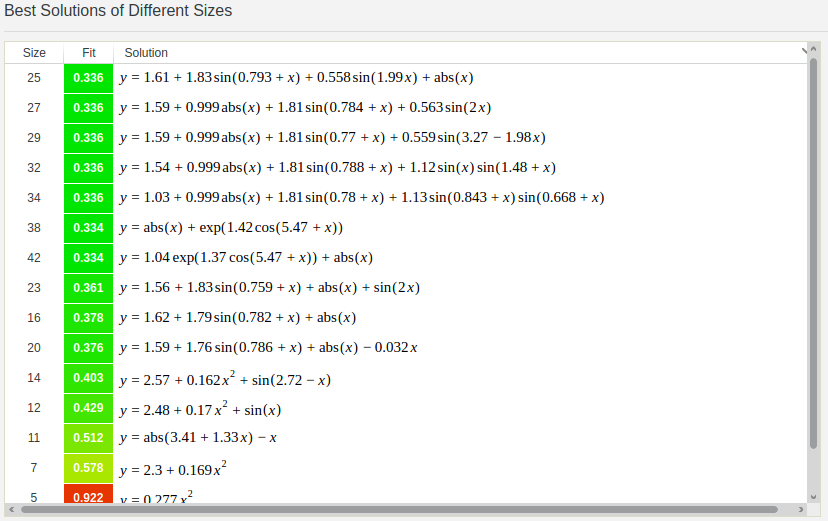
\includegraphics[width=1\linewidth]{image/best_solucao_map1_r}
		  \caption{\centering Soluções encontradas pelo software.} 
		  \label{fig:map1_solucoes_c_ruido} 
		\end{subfigure}%
		\begin{subfigure}{.55\textwidth}
		  \centering
		  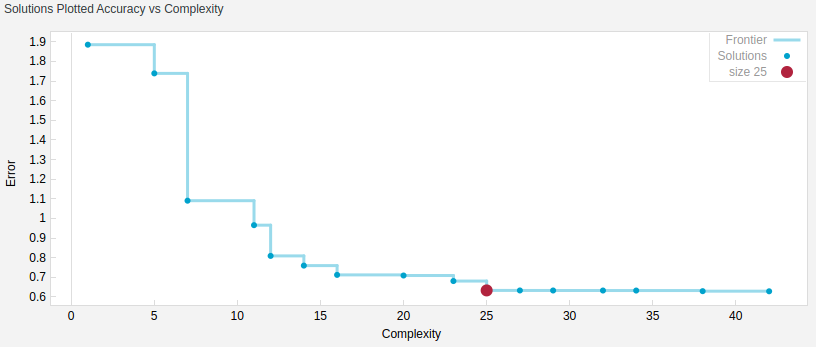
\includegraphics[width=1\linewidth]{image/pareto_map1_r}
		  \caption{\centering Compromisso acurácia \textit{x} simplicidade das
		  soluções.}
		  \label{fig:map1_pareto_c_ruido} 
		\end{subfigure}
	
		\begin{subfigure}{.5\textwidth}
		  \centering
		  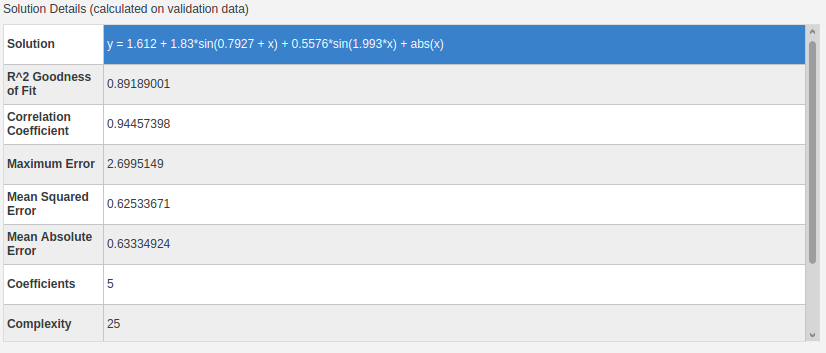
\includegraphics[width=1\linewidth]{image/best_solucao_map1_r_info}
		  \caption{\centering Resumo da melhor solução encontrada.}
		  \label{fig:map1_best_c_ruido} 
		\end{subfigure} %
		\begin{subfigure}{.45\textwidth}
		  \centering
		  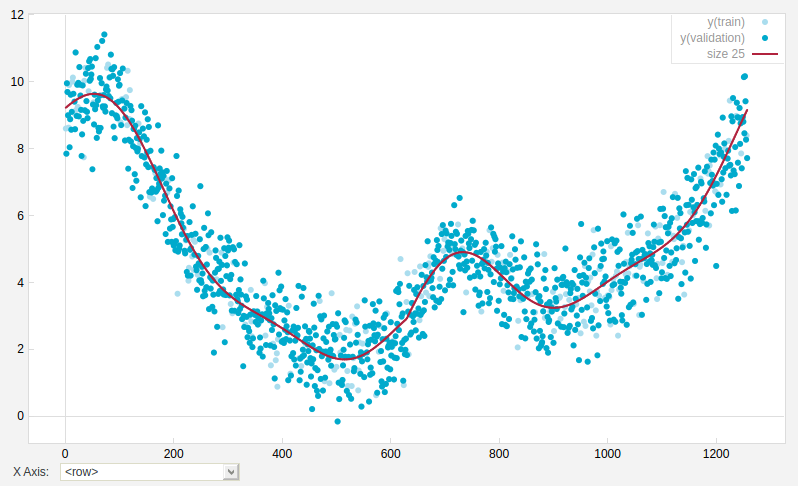
\includegraphics[width=1\linewidth]{image/solucoes_map1_r}
		  \caption{\centering Resumo do mapeamento encontrado e amostras usadas para
		  treinamento e validação.}
		  \label{fig:map1_c_ruido} 
		\end{subfigure}
	
	\caption{Resultados para mapeamento da função \ref{eq:map1} com ruídos.}
	\end{figure}
	
	\FloatBarrier

\subsection {Mapeamento y = f(x\textsubscript{1}, x\textsubscript{2},
x\textsubscript{3})}

A função escolhida para este caso está representada pela equação \ref{eq:map2},
sendo que \(x_1 \in [-3, 1]\), \(x_2 \in [1, 5]\) e \(x_3 \in [-4, 4]\). As duas
primeiras variáveis foram amostradas a cada 0.01 e a segunda, 0.02. Temos,
portanto, 401 amostras no total.

\begin{equation}
y = x_1*\log_{\pi}\left( \frac{x_2}{3}  \right) + \sqrt{2}*x_3 = 
x_1*\frac{\log_{10}\left( \frac{x_2}{3}  \right)}{\log_{10}(\pi)} + \sqrt{2}*x_3
\label{eq:map2}
\end{equation}

O mapeamento produzido pela simulação utilizando os dados sem ruídos
foi 

\begin{equation}
y =  0.959713 + 0.93436*x_3 + 0.873569*x_1*\log_{10}(x_2)
\label{eq:map2_s}
\end{equation}

O mapeamento produzido não corresponde ao utilizado para a geração dos dados,
porém os erros associados ao primeiro são praticamente nulos, isto é, o maior
erro é da ordem de \(10^{-15}\), conforme figura \ref{fig:map2_best_s_ruido}.
Isto indica que, para os os intervalos considerados para as variáveis, alguns
termos podem ser substituídos por outros sem perdas de precisão. Nota-se também,
pela figura \ref{fig:map2_solucoes_s_ruido}, que menos soluções foram encontradas em relação ao
item anterior. A imagem \ref{fig:map2_pareto_s_ruido} mostra o compromisso entre
erro e complexidade da melhor solução e é possível concluir, a partir desta
imagem, que realmente a solução de complexidade 15 supera as demais.

\FloatBarrier
			    
	\begin{figure}[h!]
	
	\centering
	
		\begin{subfigure}{.45\textwidth} 
		  \centering
		  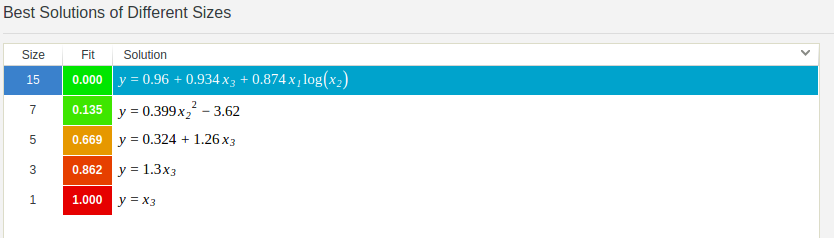
\includegraphics[width=1\linewidth]{image/solucoes_map2}
		  \caption{\centering Soluções encontradas pelo software.} 
		  \label{fig:map2_solucoes_s_ruido} 
		\end{subfigure}%
		\begin{subfigure}{.55\textwidth}
		  \centering
		  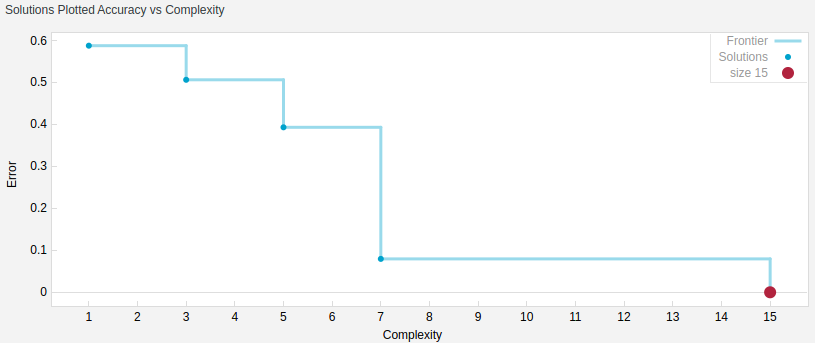
\includegraphics[width=1\linewidth]{image/pareto_map2}
		  \caption{\centering Compromisso acurácia \textit{x} simplicidade das
		  soluções.}
		  \label{fig:map2_pareto_s_ruido} 
		\end{subfigure}
	
		\begin{subfigure}{.65\textwidth}
		  \centering
		  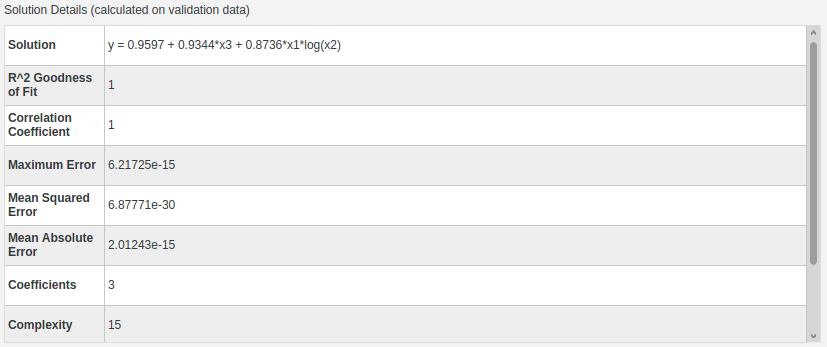
\includegraphics[width=1\linewidth]{image/best_solucao_map2_info}
		  \caption{\centering Resumo da melhor solução encontrada.}
		  \label{fig:map2_best_s_ruido} 
		\end{subfigure}
	
	\caption{Resultados para mapeamento da função \ref{eq:map2} sem ruídos.}
	\end{figure}
	
	\FloatBarrier

Enfim, a execução para os dados com ruídos gera o mapeamento 

\begin{equation}
y = 0.39025*x_2^2 - 3.555333
\label{eq:map2_r}
\end{equation}

Observa-se que \(y\) não depende de \(x_1\) e \(x_3\) neste caso. As figuras a
seguir foram geradas pelo \textit{software}. Destacam-se os seguintes fatos:

\begin{itemize}
  \item A figura \ref{fig:map2_pareto_c_ruido} mostra o compromisso entre erro e
  complexidade para as melhores soluções. Nota-se que, apesar de a solução não
  apresentar o menor erro, ela possui uma maior simplicidade comparada às
  demais. Sendo assim, ela é escolhida como a melhor solução atendendo aos
  critérios de acurácia e complexidade simultaneamente.
  \item Conforme figura \ref{fig:map2_best_c_ruido}, o erro quadrático médio é
  considerável e vale, aproximadamente, 0.70.
  \item A figura \ref{fig:map2_c_ruido} representa o mapeamento e as amostras
  utilizadas. Observa-se que este mapeamento aproxima-se relativamente bem aos
  dados.
\end{itemize}

\FloatBarrier
			    
	\begin{figure}[h!]
	
	\centering
	
		\begin{subfigure}{.45\textwidth} 
		  \centering
		  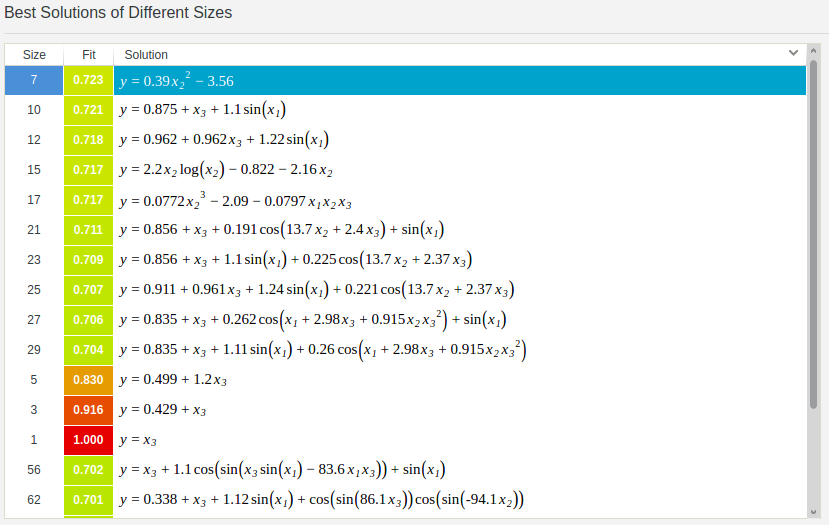
\includegraphics[width=1\linewidth]{image/solucoes_map2_r}
		  \caption{\centering Soluções encontradas pelo software.} 
		  \label{fig:map2_solucoes_c_ruido} 
		\end{subfigure}%
		\begin{subfigure}{.55\textwidth}
		  \centering
		  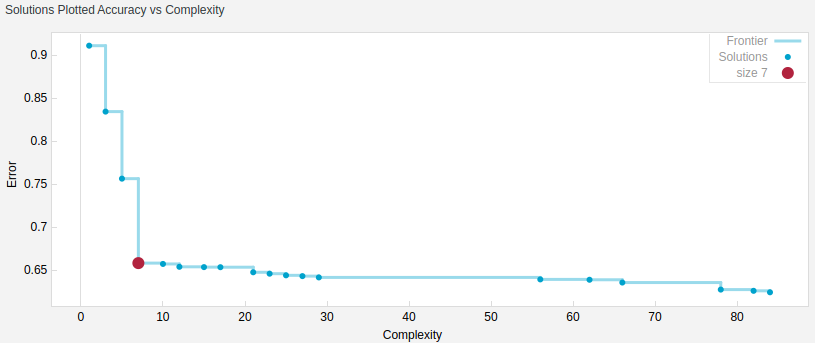
\includegraphics[width=1\linewidth]{image/pareto_map2_r}
		  \caption{\centering Compromisso acurácia \textit{x} simplicidade das
		  soluções.}
		  \label{fig:map2_pareto_c_ruido} 
		\end{subfigure}
	
		\begin{subfigure}{.5\textwidth}
		  \centering
		  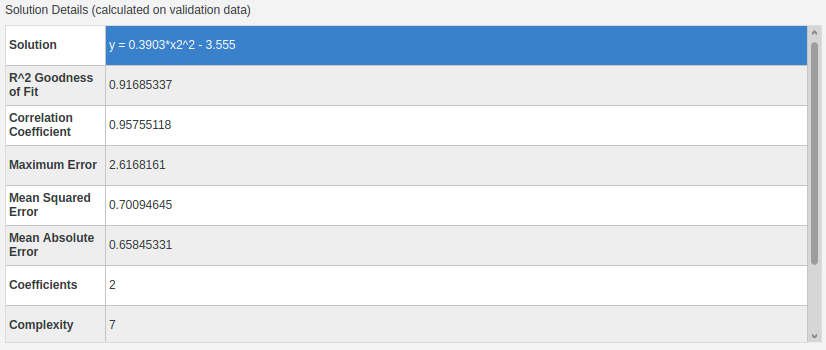
\includegraphics[width=1\linewidth]{image/best_solucao_map2_r_info}
		  \caption{\centering Resumo da melhor solução encontrada.}
		  \label{fig:map2_best_c_ruido} 
		\end{subfigure} %
		\begin{subfigure}{.45\textwidth}
		  \centering
		  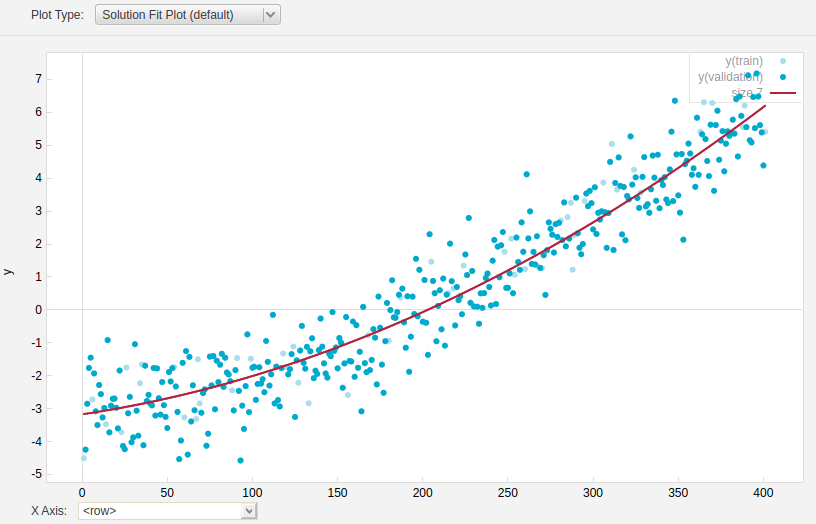
\includegraphics[width=1\linewidth]{image/best_solucao_map2_r}
		  \caption{\centering Resumo do mapeamento encontrado e amostras usadas para
		  treinamento e validação.}
		  \label{fig:map2_c_ruido} 
		\end{subfigure}
	
	\caption{Resultados para mapeamento da função \ref{eq:map2} com ruídos.}
	\end{figure}
	
	\FloatBarrier 


\section{Controle Nebuloso e Robótica Evolutiva}

\setcounter{subsection}{-1}
\subsection{Definição dos Consequentes }

O primeiro passo no controle do robô é a definição dos consequentes das regras
que serão levadas em conta. Considerando que o robô dispõe de 3 sensores
(\(d_1\), \(d_2\) e \(d_3\)) e que as funções de pertinência associadas às
medidas realizadas por eles estão representadas na seção 3 do enunciado, sugestões de consequentes estão
representadas na tabela \ref{tab:consequentes}, logo abaixo. As regras são da
forma \textbf{SE (\(d_1\) É x) E (\(d_2\) É y) E (\(d_3\) É z) ENTÃO
(\(\Delta \theta\) É w)}.

				\begin{table}[H]
					\centering
					\caption{\label{tab:consequentes} Regras que controlarão o robô.}
					\setlength\tabcolsep{4pt}
					\begin{minipage}{0.30\textwidth}
					    \centering
						\begin{tabular}{| c | c | c | c |} 
						\hline
						\(d_1\) & \(d_2\) & \(d_3\) & \(\Delta \theta\) \\ \hline
						P & MP & P & MN  \\ \hline
						P & MP & M & MN \\ \hline
						P & MP & G & MN \\ \hline
						P & PP & P & Z  \\ \hline
						P & PP & M & MN \\ \hline
						P & PP & G & MN \\ \hline
						P & PG & P & Z  \\ \hline
						P & PG & M & MN \\ \hline
						P & PG & G & MN \\ \hline
						P & MG & P & Z  \\ \hline
						P & MG & M & PN \\ \hline
						P & MG & G & MN \\ \hline
						\end{tabular}	
					\end{minipage}	      
					\begin{minipage}{0.30\textwidth}
					    \centering
						\begin{tabular}{| c | c | c | c |} 
						\hline
						\(d_1\) & \(d_2\) & \(d_3\) & \(\Delta \theta\) \\ \hline
						M & MP & P & PP \\ \hline
						M & MP & M & MP \\ \hline
						M & MP & G & MN \\ \hline
						M & PP & P & PP \\ \hline
						M & PP & M & Z  \\ \hline
						M & PP & G & PN \\ \hline
						M & PG & P & PP \\ \hline
						M & PG & M & Z  \\ \hline
						M & PG & G & PN \\ \hline
						M & MG & P & PP \\ \hline
						M & MG & M & Z  \\ \hline
						M & MG & G & PN \\ \hline
						\end{tabular}	
					\end{minipage}	
					\begin{minipage}{0.30\textwidth}
					    \centering
						\begin{tabular}{| c | c | c | c |} 
						\hline
						\(d_1\) & \(d_2\) & \(d_3\) & \(\Delta \theta\) \\ \hline
						G & MP & P & MP \\ \hline
						G & MP & M & MP \\ \hline
						G & MP & G & MP \\ \hline
						G & PP & P & MP \\ \hline
						G & PP & M & MP \\ \hline
						G & PP & G & MP  \\ \hline 	  	 
						G & PG & P & MP \\ \hline
						G & PG & M & PP \\ \hline
						G & PG & G & Z  \\ \hline
						G & MG & P & MP \\ \hline
						G & MG & M & PP \\ \hline
						G & MG & G & Z  \\ \hline
						\end{tabular}	
					\end{minipage}	      
			    \end{table}
	\FloatBarrier
	
	\subsection{Controlando o Robô}
	
	Uma vez definidas as regras que deverão ser seguidas, o próximo passo é então
	simular o comportamento do robô através do \textit{software} MATLAB. Para isso,
	5 funções foram escritas. A primeira, chamada \texttt{trap\_pertinencia},
	recebe 6 parâmetros, sendo eles a coordenada \(x\), as informações \(a\), \(b\), \(c\)
	e \(d\) referentes os trapézios que compõem as funções de pertinência e o valor
	a ser considerado caso \(x\) esteja fora do intervalo \(\left[a, d\right]\), e
	retorna o respectivo valor da função de pertinência. O programa
	\ref{lst:trap_pertinencia} abaixo possui a implementação da respectiva
	função.
	
	\lstinputlisting [language=Matlab, caption={ \texttt{trap\_pertinencia.m} -
	Avalia pertinência de um regra em função de \(x\).},
	label={lst:trap_pertinencia}] {image/trap_pertinencia.m}
	
	\vspace{12pt}
	
	A segunda função, chamada de \texttt{get\_D1\_D3\_Rule} e representada pelo
	programa \ref{lst:d1d3}, calcula a pertinência de cada um dos possíveis estados
	referentes aos sensores \(D_1\) e \(D_3\).	Essa função recebe como parâmetro a
	distância medida pelo sensor e retorna um vetor com três valores contendo a
	pertinência para os estados \textbf{P}, \textbf{M} e \textbf{G}. 
	
	\lstinputlisting [language=Matlab, caption={
	Avalia pertinência da regras de \(D_1\) e \(D_3\) em função das distâncias
	medidas.}, label={lst:d1d3}] {image/get_D1_D3_Rule.m}

	\vspace{12pt}
	
	A função \texttt{get\_D2\_Rule} realiza o mesmo que o descrito anteriormente,
	mas agora com o sensor \(D_2\). A implementação desta função pode ser
	encontrada logo abaixo.
	
	\lstinputlisting [language=Matlab, caption={
	Avalia pertinência da regras de \(D_2\) em função das distâncias
	medidas.}, label={lst:d2}] {image/get_D2_Rule.m} 
	
	\vspace{12pt}
	
	A quarta função, \texttt{get\_Angle\_Rule}, implementa as regras descritas na
	tabela \ref{tab:consequentes}. Por ser extensa, a sua implementação foi
	colocada na seção \textbf{Anexos} ao fim deste documento no programa
	\ref{lst:angle_rule}. Em poucas palavras, esta função testa se cada uma das
	regras está ativa e, caso uma determinada regra esteja, atribui a ela o menor
	valor dentre as pertinências dos estados que a compõem. Por exemplo, se \(D_1\)
	é \textbf{P} com 50\%, \(D_2\) é \textbf{MG} com 100\% e \(D_3\) é \textbf{M}
	com 33\%, então \(\Delta \theta\) é \textbf{PN} com 33\%.
	
	\vspace{12pt}
	
	A quinta função, \texttt{get\_Angle}, é responsável pelo processo de
	\textit{defuzzyficação} e está representada pelo programa \ref{lst:angle}. Ela
	utiliza o método de centro de massa para determinar \(\Delta \theta\) que
	melhor convém dadas as regras ativas.
	
	\lstinputlisting [language=Matlab, caption={
	Avalia pertinência da regras de \(D_2\) em função das distâncias
	medidas.}, label={lst:angle}] {image/get_Angle.m}
	
	\vspace{12pt}
	
	Enfim, a sexta função, \texttt{robot\_control}, realiza o controle do robô
	conforme regras especificadas acima. Sua implementação está representada pelo
	programa \ref{lst:control}.
	
	\lstinputlisting [language=Matlab, caption={  
	Automatiza controle do robô.}, label={lst:control}] {image/robot_control.m}  
	
	\subsection {Resultados}
	
	A fim de testar o controlador implementado na seção anterior, dois mapas foram
	criados. Os resultados das execuções estão representados na figuras
	\ref{fig:test_fuzzy_1} e \ref{fig:test_fuzzy_2}, em que a trajetória está
	representada em preto, a parede em cinza claro, os pontos de destino em cinza
	escuro e as posições livres, em branco. Para ambos, a direção inicial do robô é
	\(\frac{\pi}{2}\), as coordenadas iniciais são \((3,3)\) e a velocidade é \(v =
	1 \) \textit{pixel/iteração}. Verifica-se que o controle é bem-sucedido, sendo
	que o robô é capaz de realizar as curvas presentes nos mapas. É importante
	comentar que os cantos \textit{suavizados} possuem uma grande importância para o
	bom resultado, uma vez que o controle nas áreas de ``ponta'' não é tão eficiente
	visto que, quando o controlador verifica a proximidade a uma parede, ele pode
	não saber para que lado virar.
		
	\FloatBarrier
			    
	\begin{figure}[h!]
	
	\centering
	
		\begin{subfigure}{.5\textwidth}
		  \centering
		  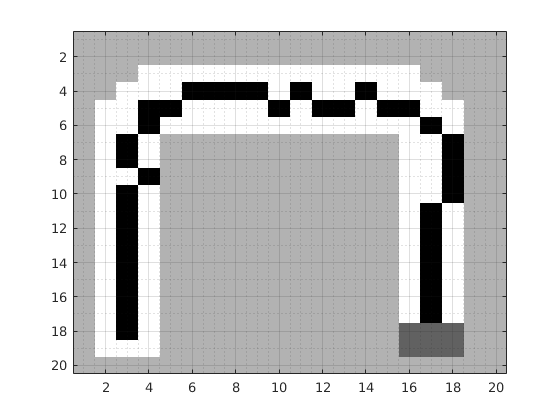
\includegraphics[width=1\linewidth]{image/test1}
		  \caption{\centering Controle do robô no mapa 1.}
		  \label{fig:test_fuzzy_1}
		  
		\end{subfigure}%
		\begin{subfigure}{.5\textwidth}
		  \centering
		  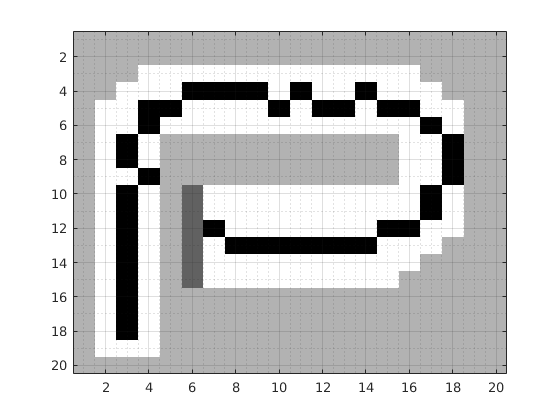
\includegraphics[width=1\linewidth]{image/test2}
		  \caption{\centering Controle do robô no mapa 2.}
		  \label{fig:test_fuzzy_2} 
		\end{subfigure}
	
	
	\caption{Resultados para o controle nebuloso do robô
	para dois mapas distintos.}
	\end{figure} 
	
	\FloatBarrier
		
	O \textit{script} utilizado nos testes pode ser encontrado no programa
	\ref{lst:test_fuzzy}.
	
	\lstinputlisting [language=Matlab, caption={  
	\textit{Script} de teste..}, label={lst:test_fuzzy}]
	{image/test_robot_control.m}

	\subsection {Controle via Rede Neural MLP}
	
	A adaptação do controle do robô via redes neurais exigiu algumas modificações
	nos programas fornecidos anteriormente nesta seção e também no algoritmo de
	evolução fornecido pelo professor, que foi utilizado na seção \ref{sec:pid}.
	Foram utilizados, neste caso, \(N = 10\) para a camada intermediária, 100
	gerações e 100 indivíduos na população.
	
	\vspace{12pt}
	
	Para o algoritmo evolutivo, foram alteradas a função de \textit{fitness}, a
	estrutura do cromossomo e as taxas de mutação e \textit{crossover}, conforme
	explicado a seguir.
	
	\begin{itemize}
	  \item A função de \textit{fitness} utilizada foi
	  \(f_{fitness}=\frac{1}{n_{colisao} + 1}\). Logo, soluções que obtiverem
	  muitas colisões serão piores, isto é, terão um \textit{fitness} menor. A
	  linha adicionada ao código foi, portanto:
	  
\begin{lstlisting}[language=Matlab, style=nonumbers]
fitness(i,1) = 1/(colision_i + 1);
\end{lstlisting}
	
	  \item  Anteriormente, tínhamos apenas 3 parâmetros a evoluir, sendo eles
	  \(k_d\), \(k_p\) e \(k_i\). Neste caso, o número de parâmetros depende do
	  número de neurônios na camada intermediária. Sejam \(N\) neurônios nesta
	  camada, cada um deles terá 4 pesos, sendo um deles para a entrada constante e
	  o restante para as distâncias dos sensores. Há ainda mais \(N + 1\) pesos a
	  serem ajustáveis, correpondentes à soma dos resultados de cada neurônio. A
	  estrutura utilizada foi, portanto:
	  
\begin{lstlisting}[language=Matlab, style=nonumbers]
% Numero de entradas: d1, d2, d3 e termo constante
E = 3 + 1;
pop = randn(tam_pop, E * n_neurons + n_neurons + 1);
\end{lstlisting}	  
	
	  Utilizou-se também uma distribuição normal de média 0 e variância 1 para os
	  pesos iniciais da rede neural.
	  
	  \item A fim de maximizar a diversidade na rede, utilizou-se taxas de mutação
	  \(p_m = 0.8\) e \textit{crossover} \(p_c = 0.9\).

	\end{itemize}
	
	O controle do robô, realizado pela \texttt{robot\_control\_mlp}, também foi
	alterado. A linhas referentes ao controle nebuloso (linhas 75 a 86 do programa
	\ref{lst:control}) foram retiradas e substituídas pelo trecho de código abaixo.
	
\begin{lstlisting}[language=Matlab, caption={Trecho de código do controle do
robô feito via rede MLP.}, label={lst:control_mlp}] 
% Constroi vetor das entradas de cada neuronio
mlp_input = [distance_d1 distance_d2 distance_d3 1];

% middle_layer_output contera as saidas de cada neuronio da camanda
% intermediaria
middle_layer_output = zeros (1, n_neurons);

% Calcula a saida de cada neuronio. mlp_weights contem todos os pesos
% sinapticos da rede 
for n = 1 : n_neurons
    
    middle_layer_output (1, n) = ...
        tanh(mlp_input * mlp_weights (1 + (n - 1)* 4 : 4 + (n - 1)* 4)');
    
end

% a entrada da ultima camada eh a saida da camada intermediaria e uma
% termo constante.
last_layer_input = [middle_layer_output 1];

% Calcula o desvio na direcao do robo. Seleciona ultimos n_neurons + 1 pesos
% sinapticos. 
d_angle = ...
 last_layer_input * mlp_weights (1 + 4 * n_neurons : 1 + 4 * n_neurons + n_neurons)';

robot_direction = robot_direction + d_angle;

teste (round(m_length + 1 - y_robot), round(x_robot)) = 'r';

% Calcula nova posicao.
x_robot = x_robot + speed*cos(robot_direction);
y_robot = y_robot + speed*sin(robot_direction);

% Verifica se a nova posicao esta dentro do mapa.
if (round(x_robot) > length(labyrinth_matrix (1,:))) ...
        || (round(x_robot) < 1) ...
        || (round(m_length + 1 - y_robot) < 1) ...
        || (round(m_length + 1 - y_robot) > m_length)
    
    % Penalisa movimentos que levam o robo fora do mapa.
    colisions = colisions + 1000;
    
% Detecta colisao.
elseif (labyrinth_matrix (round(m_length + 1 - y_robot), round(x_robot)) == '#')
    
    % Aumenta contador de colisoes.
    colisions = colisions + 1;
end
\end{lstlisting}
	
O mapa da figura \ref{fig:test_fuzzy_2} foi utilizado no treinamento da rede
neural, visto que apresenta situações mais desafiadoras que o mapa da figura
\ref{fig:test_fuzzy_1}. Sendo assim, acredita-se que se o programa for
bem-sucedido em calcular os pesos sinápticos para o mapa mais complexo, então,
os mesmos pesos serão adequados para mapas mais simples. As figuras
\ref{fig:mlp_2} e \ref{fig:mlp_1} contém resultados para um dos vetores de
pesos sinápticos encontrado pelo algoritmo evolutivo em que essa afirmação é
comprovada.

\FloatBarrier
			    
	\begin{figure}[h!]
	
	\centering
	
		\begin{subfigure}{.5\textwidth}
		  \centering
		  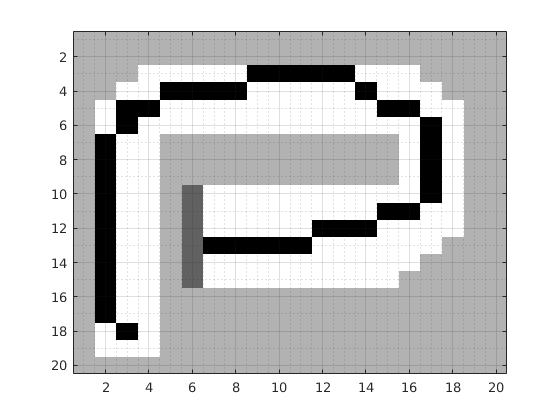
\includegraphics[width=1\linewidth]{mlp_robot/mlp_2}
		  \caption{\centering Controle do robô via MLP no mapa 2.}
		  \label{fig:mlp_2}
		  
		\end{subfigure}%
		\begin{subfigure}{.5\textwidth}
		  \centering
		  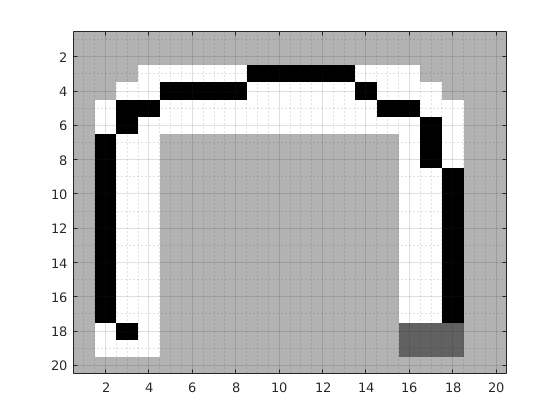
\includegraphics[width=1\linewidth]{mlp_robot/mlp_1}
		  \caption{\centering Controle do robô via MLP no mapa 1}
		  \label{fig:mlp_1} 
		\end{subfigure}
	
	
	\caption{Resultados para o controle do robô via MLP
	para dois mapas distintos.}
	\end{figure} 
	
	\FloatBarrier
	
	A figura \ref{fig:fitness_mlp} representa a evolução do \textit{fitness} ao
	decorrer da execução do algoritmo evolutivo. Verifica-se que, apesar da melhor
	solução ser encontrada nas primeiras gerações, o \textit{fitness} médio é muito
	pequeno em todas as gerações. Esse fato pode ser explicado pelos valores das
	taxas de mutação e \textit{crossover}, responsáveis por manter uma grande
	diversidade na população. Dessa forma, sempre serão adicionados à população
	indivíduos ruins, isto é, que produzem baixos \textit{fitness}.
	
	\FloatBarrier
	
	\begin{figure}[h]
    \centering
    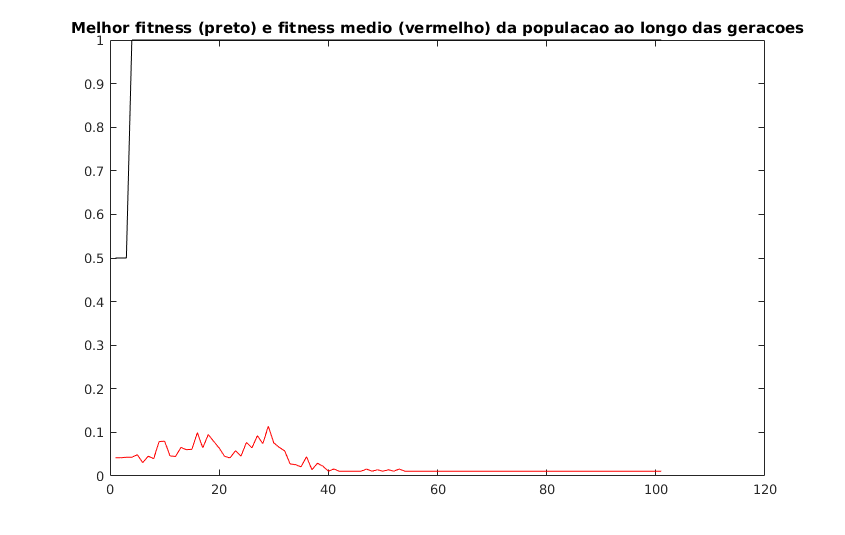
\includegraphics[scale=0.65]{mlp_robot/fitness}
    \caption{\label{fig:fitness_mlp}Evolução do \textit{fitness} médio e
    melhor.}
	\end{figure}  
	
	\FloatBarrier
	
	As figuras \ref{fig:mlp_2_1} e \ref{fig:mlp_2_2} foram obtidas pelo
	treinamento da rede neural no mapa da figura \ref{fig:test_fuzzy_1}.  
	
	\FloatBarrier
			    
	\begin{figure}[h!]
	
	\centering
	
		\begin{subfigure}{.5\textwidth}
		  \centering
		  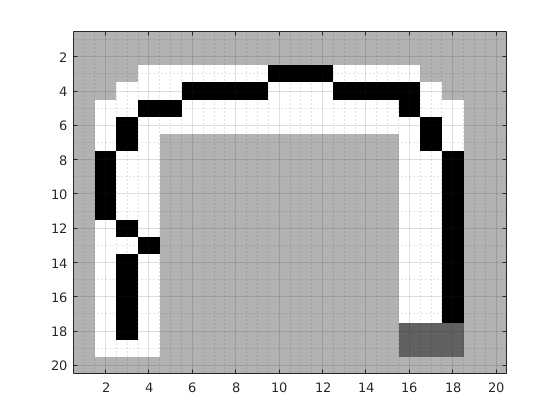
\includegraphics[width=1\linewidth]{mlp_robot/mlp_1_2}
		  \caption{\centering Controle do robô via MLP no mapa 1.}
		  \label{fig:mlp_2_1}
		  
		\end{subfigure}%
		\begin{subfigure}{.5\textwidth}
		  \centering
		  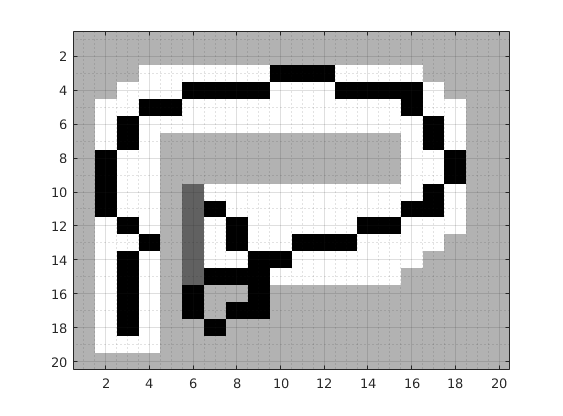
\includegraphics[width=1\linewidth]{mlp_robot/mlp_2_2}
		  \caption{\centering Controle do robô via MLP no mapa 2.}
		  \label{fig:mlp_2_2} 
		\end{subfigure}
	
	
	\caption{Resultados para o controle do robô via MLP
	para dois mapas distintos.}
	\end{figure} 
	
	\FloatBarrier
	
Verifica-se que a solução encontrada para o primeiro mapa, que é mais simples,
controla corretamente o robô. Entretanto, se o mesmo controle fosse utilizado
para o mapa 2, então o robô colidiria com a parede, conforme mostrado na figura
\ref{fig:mlp_2_2}. Isso é explicado pelo fato de que o mapa exige um controle
mais complexo que o primeiro.


\section{Sistema de recomendação empregando \textit{k}-NN}

\subsection {Abordagens \textit{User-based} e \textit{Item-based}}

De acordo com o \textit{paper} \textit{State-of-the-art Recommender Systems},
sistemas de recomendação que utilizam a abordagem \textit{user-based} exploram
as similaridades entre usuários que possuam características em comum para
predizer uma classificação que um usuário faria potencialmente para um item.
Sendo assim, define-se o conjunto \(\mathbb{U}\) formado pelos usuários , o
conjunto \(\mathbb{I}\) formado pelos itens e  o conjunto \(\mathbb{R}\) que
possui todas as classificações dadas.  Uma classificação \(r_{ui}\) é dada pelo
usuário \(u\in \mathbb{U}\) para o item \(i\in \mathbb{I}\)  e cada usuário
\(u\) possui um conjunto de itens avaliados \(\mathbb{S}_u \subseteq
\mathbb{I}\). A predição da classificação que um usuário \(a\in\mathbb{U}\)
faria para o item \(i \notin \mathbb{S}_a\) e que considere \(K\) elementos do
conjunto \(\mathbb{T}_a\), que contém \(K\) outros usuários cujas
preferências sejam as mais parecidas com as de \(a\), é então:

\begin{equation}
p_{ai} = \frac{\sum_{\{ u\in \mathbb{T}_a | i\in \mathbb{S}_u \}} \left(
sim(a,u) * r_{ui} \right)}{\sum_{\{ u\in \mathbb{T}_a | i\in \mathbb{S}_u \}}
\left| sim(a,u)\right|}
\end{equation}

ou

\begin{equation}
p_{ai} = \bar{r_a} + \frac{\sum_{\{ u\in \mathbb{T}_a | i\in \mathbb{S}_u \}}
\left( sim(a,u) * (r_{ui} - \bar{r_u})\right)}{\sum_{\{ u\in \mathbb{T}_a | i\in
\mathbb{S}_u \}} \left| sim(a,u)\right|}
\end{equation}

em que \(sim(a,u)\) mede o grau de similaridade entre \(a\) e \(u\) e
\(\bar{r_v}\) é a média das classificações de um usuário \(v\). A segunda
expressão leva em consideração as diferenças de intensidade entre os usuários
(por exemplo, em um sistema de 0 a 5, para \(u\), \textit{muito bom} pode ser
3.5, mas, para \(a\), isso é 5) Essas equações nos dizem, portanto, que a
predição realizada se aproximará da classificação feita pelo usuário \(u\) cujas
características são as mais parecidas em relação a aquelas de \(a\).

\vspace{12pt}

A abordagem \textit{item-based}, por sua vez, utiliza os \textit{ratings} de
itens \(j\) já classificados pelo usuário para predizer a possível classificação
que o respectivo usuário daria a um item \(i\), dado o grau de semelhança entre este
item não avaliado e aqueles avaliados. Define-se também a vizinhança
\(\mathbb{T}_i\), contendo \(K\) itens próximos de \(i\) em termos de
características. Assim como no caso anterior, essa predição \(p_{ai}\) pode ser
realizada de duas maneiras:


\begin{equation}
p_{ai} = \frac{\sum_{\{ j\in \mathbb{S}_a \cap \mathbb{T}_i \}} \left(
sim(i,j) * r_{aj} \right)}{\sum_{\{ j\in \mathbb{S}_a \cap \mathbb{T}_i \}}
\left| sim(i,j)\right|}
\end{equation}

ou

\begin{equation}
p_{ai} = \bar{r_i} + \frac{\sum_{\{ j\in \mathbb{S}_a \cap \mathbb{T}_i \}}
\left( sim(i,j) * (r_{aj} - \bar{r_j})\right)}{\sum_{\{ j\in \mathbb{S}_a \cap
\mathbb{T}_i \}} \left| sim(i,j)\right|}
\end{equation}

em que \(sim(i,j)\) mede o grau de similaridade entre os itens \(i\) e \(j\) e
\(\bar{r_k}\) é a média das classificações feitas para o item \(k\). Como na
abordagem anterior, considera-se que itens muito parecidos terão
\textit{ratings} também muito parecidos.

\subsection{Exemplo de Aplicação}
 
Utilizando o programa \texttt{exemplo.m} como referência e o \textit{toolbox}
fornecido, foi possível implementar a função \texttt{movieLens\_impute\_data},
representada pelo programa \ref{lst:movielens} logo abaixo. A função define um
usuário, cuja identificação está contida na variável \texttt{user\_id}, para
qual serão calculadas as respectivas recomendações. O programa possui também
outro parâmetro, chamado \texttt{k\_neighbors}, que define a quantidade de
vizinhos que serão utilizados no cálculo. Ao final, são impressas as
recomendações encontradas e os \textit{ratings} dos vizinhos mais próximos do
usuário.

\lstinputlisting [language=Matlab, caption={
	Recomenda filmes para um data usuário segundo o método kNN.},
	label={lst:movielens}] {kNN/movieLens_impute_data.m}
 
\vspace{12pt}
 
Os resultados da execução do programa acima estão representados nas tabelas
abaixo. Foi escolhido aleatoriamente o usuário 898 e foram utilizados os 3
vizinhos mais próximos. No bloco superior da coluna da esquerda, estão
representadas as recomendações calculadas e que foram bem-sucedidas, isto é, as
recomendações que a função \texttt{knnImputeRo.m} não retornou como
\textit{NaN}. Observa-se que os filmes para os quais uma recomendação foi
calculada devem possuir ao menos uma \textit{rating} não nula em algum dos
dos vizinhos. Caso contrário, não haveria dados suficientes para o cálculo das
respectivas predições. Nos outros 3 blocos estão contidos as \textit{ratings}
realizadas pelos vizinhos, em ordem de semelhança com o usuário. Por exemplo, o
vizinho 408 possui uma semelhança de 64.8\% com o usuário e assim por diante.

\vspace{12pt}
 
É possível alguns fatos:

\begin{itemize}
  \item O item 294 foi classificado por 408 e 205, sendo que o primeiro possui
  uma semelhança de 64.8\% com o usuário 898 e o segundo, apenas 20.6\%. 408 deu
  a pontuação máxima, enquanto 205 deu apenas uma nota 3.0. A nota recomendada
  para 898 foi 4.49, que é muito mais próxima de 5 do que de 3. Esse resultado
  está correta, visto que 408 é muito mais semelhante a 898 do que 205 e,
  portanto, espera-se que eles dêem notas parecidas.

  \item  O item 1025 só foi avaliado por 205, que não possui uma grande
  semelhança com 898. A nota recomendada estará, portanto, ao redor do
  \textit{rating} feito por 205, mas possuirá uma pequena margem que levará em
  conta essa falta de \textit{total} semelhança.

  \item O item 333 foi avaliado pelos usuários 384 e 205. Ambos deram nota 4. A
  nota recomendada para 898 deve ser, portanto, muito próxima de 4, já que dois
  outros vizinhos deram a mesma nota. Observa-se justamente este fato: a nota
  recomendada para 898 é 3.99.
\end{itemize} 

 
\begin{minipage} {0.45\textwidth}
\begin{lstlisting}[style=nonumbers]
=============================
Estimativas para usuario 898
=============================
Recomendacao para filme 268 : 2.64
Recomendacao para filme 269 : 3.64
Recomendacao para filme 289 : 4.50
Recomendacao para filme 294 : 4.49
Recomendacao para filme 304 : 3.64
Recomendacao para filme 322 : 3.64
Recomendacao para filme 326 : 4.64
Recomendacao para filme 329 : 2.36
Recomendacao para filme 333 : 3.99
Recomendacao para filme 355 : 3.36
Recomendacao para filme 678 : 1.64
Recomendacao para filme 875 : 2.64
Recomendacao para filme 878 : 3.36
Recomendacao para filme 879 : 3.36
Recomendacao para filme 984 : 1.64
Recomendacao para filme 989 : 3.36
Recomendacao para filme 1025 : 1.64
\end{lstlisting}

\begin{lstlisting}[style=nonumbers]
=============================
Ratings do usuario 408 
de maior similaridade (0.648)
=============================
Rating para filme 294 : 5.00
\end{lstlisting}
\end{minipage} \hspace{0.03\textwidth}% 
\begin{minipage} {0.45\textwidth}
\begin{lstlisting}[style=nonumbers]
=============================
Ratings do usuario 384
 de maior similaridade (0.212)
=============================
Rating para filme 289 : 5.00
Rating para filme 329 : 3.00
Rating para filme 333 : 4.00
Rating para filme 355 : 4.00
Rating para filme 878 : 4.00
Rating para filme 879 : 4.00
Rating para filme 989 : 4.00
\end{lstlisting}

\begin{lstlisting}[style=nonumbers]
=============================
Ratings do usuario 205
de maior similaridade (0.206)
=============================
Rating para filme 268 : 2.00
Rating para filme 269 : 3.00
Rating para filme 289 : 4.00
Rating para filme 294 : 3.00
Rating para filme 304 : 3.00
Rating para filme 322 : 3.00
Rating para filme 326 : 4.00
Rating para filme 333 : 4.00
Rating para filme 678 : 1.00
Rating para filme 875 : 2.00
Rating para filme 984 : 1.00
Rating para filme 1025 : 1.00
\end{lstlisting}
\end{minipage}


\section{Sistema de recomendação – Paradigma alternativo}

\subsection{Funcionamento do SCOAL}

Conforme explorado na seção anterior, o algoritmo \textit{k-NN} primeiramente
divide a matriz de dados em \textit{co-clusters} e, em seguida, realiza uma
predição baseada em um desses \textit{co-clusters} gerados. Tal algoritmo,
portanto, não leva em consideração os atributos dos filmes e dos usuários, isto
é, a predição é baseada exclusivamente nos \textit{ratings} dos usuários em uma
vizinhança. O algoritmo \textit{SCOAL}, por sua vez, utiliza ambas as
informações de vizinhança e atributos para predizer uma nota. A ideia do
\textit{SCOAL} é dividir toda a matriz em grupos, ou \textit{clusters}, de
maneira que cada um possa ser bem caracterizado por um único modelo preditivo. A
similaridade é dada, portanto, pela similiridade dos modelos preditivos e não
somente dos valores dos \textit{ratings}, como acontece no \textit{k-NN}. Além
disso, o \textit{SCOAL} realiza o agrupamento, ou \textit{co-clustering}, simultaneamente
com a obtenção dos respectivos modelos de classificação, a fim de melhorar a
designação dos dados aos \textit{clusters} e a precisão dos modelos.

\subsection{A base de dados \textit{MovieLens}}

Os dados utilizados nesta seção foram disponibilizados pelo grupo
\textit{GroupLens} no mês de Abril de 1998. São 100.000 \textit{ratings},
compreendidas no intervalo \([1,5]\), dadas por 943 usuários em 1682 filmes e
coletadas durante 7 meses, indo de 19 de setembro de 1997 até 22 de abril de
1998. É importante dizer que esses dados foram filtrados, de forma que usuários
com menos de 20 \textit{ratings} ou que não possuíssem informações
demográficas completas foram eliminados da base. Essas informações demográficas
são compostas por idade, sexo, ocupação e endereço \textit{zip}. Filmes, além
de informações sobre título, data de lançamento e \textit{url} do IMDb,
podem possuir diversos gêneros (ação, comédia, aventura etc). Destaca-se também
que a matriz é muito esparsa, isto é, muito de seus campos não estão
preenchidos.

\vspace{12pt}

Esses dados foram disponibilizados em alguns arquivos, cujos os principais são:

\begin{itemize}
  \item \texttt{u.data}: arquivo contendo as classificações dos usuários. Cada
  linha, além de possuir a respectiva \textit{rating}, associa um \textit{id} de
  usuário a um \textit{id} de filme. Adicionalmente, há um outro atribuot que
  descreve a data que a respectiva classificação foi dada.

  \item \texttt{u.item}: possui as informações apresentadas acima sobre os
  filmes.
  
  \item \texttt{u.user}: possui as informações apresentadas acima sobre os
  usuários.
  
\end{itemize}

\subsection{Execução do \textit{toolbox} fornecido}

O programa fornecido foi executado com 5 pastas para a \textit{k-fold
cross-validation}, 3 cortes nas linhas e 3 cortes nas colunas.
Foram gerados, portanto, 16 \textit{co-clusters}. Os coeficientes presentes na
tabela \ref{scoal:coef} foram obtidos para a iteração que apresentou menor MSE
(\textit{Mean Squared Error}). A imagem \ref{fig:scoal_result} representa o
valor deste indicador juntamente com alguns outros que avaliam o desempenho dos
preditores gerados, como. por exemplo, \textit{Precision} e \textit{Recall}. 

\FloatBarrier
	
	\begin{figure}[h]
    \centering
    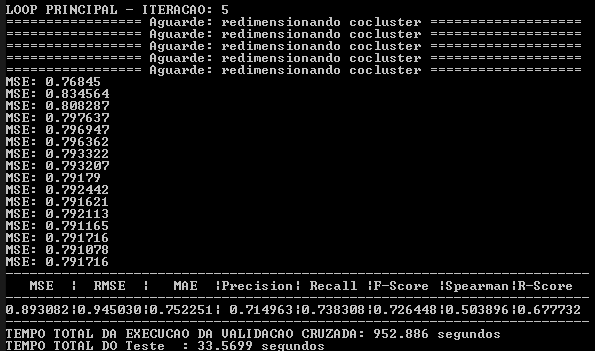
\includegraphics[scale=0.65]{scoal/execucaoScoal}
    \caption{\label{fig:scoal_result}Resultados para a 5ª iteração do
    algoritmo.}
	\end{figure}  
	
\FloatBarrier

\FloatBarrier
{\footnotesize
\begin{longtable}[h]{| c | p{0.9\textwidth} |} 

	\caption{\label{scoal:coef} Modelos preditivos para cada \textit{co-cluster}
	na iteração 5.}	\\
					
	\hline
	\textbf{Modelo} & \textbf{Coeficientes} \\ \hhline{|=|=|}
	1 & 0.145453; -0.305456; 0.041422; 0.118563; -0.100787; 0.100787; -0.361339;
	 -0.031360; -0.145453; 0.052350; 0.021124; 0.011262; 0.010038;
	-0.538674; -0.047585; -0.572105; -0.092489; -0.080133; -0.055039; -0.489122; 0.022816;
	-0.356975; -0.083862; 0.036848; 0.130115; -0.112789; -0.080782; 0.148531;
	-0.145453; 0.017635; 0.019313; -0.042312; 0.032170; 0.011268; -0.01965;
	0.037008; 0.027218; -0.003466; -0.055387; 0.006280; -0.039053; 0.006584;
	0.015461; -0.006752; -0.002389; 0.017252; -0.018370; -0.077912; 1.871064;
	-0.000088; \\ \hline
	2 & 0.158438; 0.098412; -0.084444; -0.172333; 0.098928; -0.098928; 0.114960;
	-0.237276; -0.033229; -0.216696; -0.133264; 0.131348; -0.468453; -0.232276;
	0.136819; -0.104005; -0.296712; -0.018775; 0.036848; -0.123124; -0.286383;
	-0.046800; -0.222357; -0.032034; -0.350149; -0.169591; -0.458762;
	-0.010351; -0.158438; 0.024304; 0.017394; 0.003218; -0.040178; -0.006777;
	-0.008178; 0.165993; -0.026013; -0.024336; 0.019608; -0.019747; 0.082755;
	-0.050241; 0.009563; 0.023744; 0.006748; -0.006169; -0.021861; -0.010928;
	1.978979; -0.338162; \\ \hline
	3 & 0.154957; 0.140657; -0.130708; -0.164910; -0.001337; 0.001337;
	-0.107116; -0.486860; -0.235860; -0.210768; -0.361360; -0.228055; -0.126928;
	0.125811; -0.027875; -0.081434; -0.067236; -0.402994; -0.304448; 0.082657;
	0.055919; -0.188501; 0.159001; -0.225646; -0.062895; -0.278069; 0.027141;
	0.036943; -0.154957; 0.013116; 0.003827; -0.004108; -0.055794; -0.003045;
	-0.009006; -0.125374; -0.004883; 0.011032; -0.000223; 0.036841; 0.004948;
	0.045497; -0.000247; -0.016238; 0.028038; 0.004095; 0.044256; 0.004544;
	1.914104; -0.363268 ; \\ \hline 
	4 & 0.160529; 0.007257; -0.117741; -0.050074; -0.018830; 0.018830; -0.112880;
	-0.150154; 0.128904; -0.145439; -0.064703; -0.187139; -0.365357; -0.049431;
	-0.576610; -0.005741; -0.242354; -0.274566; 0.188305; -0.146628; -0.154143;
	-0.511182; 0.103514; -0.154050; -0.053636; 0.063296; -0.346568; -0.294042;
	-0.160529; -0.062514; -0.033490; 0.011760; -0.009649; 0.028094; 0.037871;
	0.019659; 0.037787; 0.081594; 0.027281; 0.011614; 0.008447; -0.025850;
	-0.015608; -0.000924; -0.032736; -0.015211; -0.009934; 0.041682; 2.259185;
	0.176226; \\ \hline 
	5 & 0.153238; -0.289953; 0.056217; 0.080444; -0.176394;
	0.176394; -0.272798; -0.345049; -0.153238; 0.060464; 0.061706; -0.235400;
	0.112666; -0.929689; -0.127659; -0.791338; 0.004033; -0.168081; -0.072029;
	-0.360590; 0.142148; -0.094107; -0.204140; 0.150260; 0.112863; -0.007595;
	0.204809; 0.205846; -0.153238; 0.012859; -0.017582; -0.033241; 0.029942;
	-0.022328; -0.018988; -0.081810; -0.009810; 0.120705; -0.081946; 0.167287;
	-0.059177; 0.000068; 0.000693; 0.030118; 0.025867; -0.000215; -0.026430;
	0.026859; 2.078046; 0.163905; \\ \hline 
	6 & 0.209385; -0.615300; 0.275593;
	0.130311; -0.269474; 0.269474; -0.166631; -0.324050; -0.209385; 0.314726;
	-0.031355; -0.600633; 0.233076; 0.036878; -0.645836; -0.776475; -0.369757;
	0.416463; -0.554884; -0.567367; 0.048666; 0.463706; -0.531050; -0.209385;
	0.149720; -0.001071; -0.654194; 0.093764; -0.209385; 0.130455; 0.056835;
	-0.222108; 0.086176; 0.011397; 0.352807; 0.090408; -0.099081; -0.172382;
	-0.283249; 0.001985; 0.146003; 0.214892; -0.122668; 0.044627; -0.096482;
	0.454269; 0.216841; 0.011747; 1.363391; 0.286857; \\ \hline 
	7 & 0.074156;
	-0.276172; 0.156241; 0.045794; -0.153727; 0.153727; -0.169476; 0.292783;
	-0.074156; 0.281942; 0.060345; -0.116324; -0.031924; -0.460518; -0.364804;
	-0.150334; 0.081755; 0.013356; 0.034094; -0.531589; 0.069247; 0.279620;
	-0.135149; -0.477126; 0.135330; -0.167795; 0.021751; 0.169321; 0.059546;
	0.140365; 0.112379; -0.142606; 0.132601; 0.024045; 0.082573; -0.056270;
	0.040479; -0.828516; -0.107644; 0.012118; -0.106625; -0.063357; 0.015247;
	0.098645; 0.052261; 0.196016; -0.317204; -1.302668; 1.844769; 0.773247;\\ \hline
	8 & 0.159554; 0.130232; -0.149348; -0.140438; 0.071082; -0.071082; 0.079011;
	0.161992; -0.059673; -0.132908; -0.259776; 0.116072; -0.766087; -0.263210;
	-0.119554; -0.139388; -0.213015; 0.004084; 0.484236; -0.130024; -0.291548;
	-0.072007; -0.454042; -0.178572; -0.410951; -0.170437; -0.215582; -0.039038;
	-0.159554; 0.063759; -0.014169; 0.026256; -0.027020; -0.000913; 0.025837;
	0.059471; -0.062676; -0.091991; -0.109653; 0.076020; 0.054455; -0.056571;
	-0.021649; -0.070765; -0.019649; 0.012628; -0.020391; 0.168960; 1.712372;
	-0.158062;\\ \hline 
	9 & 0.165744; 0.072184; -0.141980; -0.095928; -0.082982;
	0.082982; -0.186644; -0.866382; -0.170484; -0.250890; -0.399213; 0.008862;
	-0.057555; 0.085714; -0.161120; 0.336326; -0.139211; -0.276578; -0.238796;
	-0.024920; -0.014957; 0.023362; -0.160613; -0.180117; -0.088914; -0.298469;
	-0.090202; 0.055767; -0.165744; -0.038946; -0.007102; 0.101837; -0.014165;
	-0.059708; 0.001603; 0.051558; -0.014857; -0.087410; 0.053863; -0.008801;
	-0.152968; 0.007850; 0.015132; 0.039744; 0.002453; 0.034771; 0.055539;
	-0.118275; 1.708164; -0.080727; \\ \hline 
	10 & 0.117609; 0.121627; -0.282165;
	0.042916; -0.058406; 0.058406; 0.107498; -0.117609; -0.019190; -0.405692;
	-0.273367; -0.255412; -0.549664; -0.314560; -0.176684; -0.181694; -0.070138;
	0.562161; 0.836102; -0.059110; 0.195050; 0.036555; -0.622938; 0.178962;
	-0.181715; -0.150814; -0.772024; -0.172533; -0.117609; -0.053115; 0.153536;
	0.002256; -0.200794; -0.038823; -0.042921; -0.217099; -0.032497; 0.067446;
	-0.117609; 0.036354; -0.125077; 0.375880; -0.025930; -0.304797; 0.088381;
	-0.225396; -0.092929; -0.273183; 0.864530; -0.211613;\\ \hline 
	11 & 0.075682;
	0.014163; -0.047494; -0.042352; -0.113082; 0.113082; -0.050384; 0.136660;
	0.092318; 0.078522; -0.203886; 0.599453; -0.554428; 0.183884; -0.075682;
	-0.075682; -0.049259; -0.770246; 0.006306; -0.288197; -0.184931; -0.765363;
	0.041453; 0.315831; 0.098852; 0.079702; -0.052735; 0.480192; -0.075682;
	-0.180874; -0.148958; 0.356630; -0.223928; -0.082032; -0.277486; -0.068537;
	0.094255; 0.013841; -0.075682; 0.137614; 0.009946; -0.565146; -0.112763;
	-0.057013; 0.234001; 0.189301; -0.070850; -0.739999; 2.326597; 0.268200;  \\
	\hline 
	12 & 0.191561; -0.193858; 0.029130; -0.026836; 0.042587; -0.042587;
	-0.089181; 0.203084; -0.089162; -0.331050; -0.134555; -0.033791; -1.134447;
	-0.247984; -0.280799; -0.576608; -0.018402; 0.212571; 0.702313; -0.195558;
	-0.476448; 0.163142; -0.087483; -0.088211; -0.307796; -0.229101; -0.599600;
	0.064498; 0.093746; -0.011906; -0.013979; 0.111372; 0.037223; 0.008758;
	-0.065282; -0.143293; 0.016528; 0.150781; -0.044906; 0.039258; -0.196244;
	-0.079988; -0.003830; 0.047696; -0.041619; 0.218680; 0.006091; 0.417986;
	1.150833; -0.683341; \\ \hline
	13 & 0.148209; -0.059039; -0.083705; -0.005491; 0.010328; -0.010328; -0.230760;
	-0.189309; -0.538609; -0.103990; 0.219079; -0.530764; 0.356418; -0.322340;
	-0.148209; -0.368023; 0.144423; -0.091621; -0.148209; 0.105816; -0.121599;
	-0.270846; -0.081490; -0.203113; -0.148463; 0.199290; -0.343332; -0.031252;
	-0.148209; 0.040285; -0.041633; -0.027047; -0.062109; -0.001586; -0.117222;
	0.468140; 0.015223; -0.018937; 0.003423; 0.318983; -0.146294; -0.111940;
	0.022961; -0.028951; 0.099396; 0.064670; 0.151182; -0.592075; 2.222140;
	-0.427067;  \\ \hline
	14 & 0.175461; 0.036977; -0.155914; -0.056518; -0.062314; 0.062314; -0.268933;
	0.518875; -0.288730; -0.108100; -0.236450; -0.343871; 0.376072; -0.026862;
	-0.173402; 0.024717; -0.137289; -0.561450; -0.004052; -0.388198; -0.188005;
	0.063221; -0.817763; 0.035023; -0.129884; -0.356983; -0.320587; -0.060569;
	-0.440755; 0.005263; 0.151253; 0.187391; -0.000756; -0.047214; -0.044171;
	0.091214; -0.025574; -0.001232; 0.264114; -0.041650; 0.074576; 0.014387;
	-0.036335; 0.107233; -0.067227; -0.029637; -0.045870; -0.114915; 2.653960;
	0.109496; \\ \hline
	15 & 0.183501; -0.230915; 0.040334; 0.007055; -0.124662; 0.124662; -0.219916;
	-0.402084; 0.738653; -0.155448; -0.319779; -0.025436; -0.121768; -1.444828;
	-0.108418; -1.038054; -0.111564; 0.172685; -0.059428; -0.219212; -0.050784;
	-0.056240; -0.045836; -0.002217; 0.205654; 0.066217; -0.287053; -0.174689;
	0.045627; -0.023441; -0.003491; 0.187322; -0.103295; 0.034463; 0.040738;
	0.033431; 0.042559; 0.197273; -0.092128; 0.002823; -0.188358; 0.063411;
	-0.013565; 0.022282; -0.067198; -0.005062; 0.033840; 0.002839; 1.283242;
	0.430237;  \\ \hline
	16 & 0.129548; -0.192931; -0.011378; 0.074778; 0.100693; -0.100693; -0.372648;
	0.139234; 0.183694; -0.123371; 0.039792; 0.270973; 0.124380; -0.287096;
	-0.129548; -0.449262; 0.088444; -0.109449; -0.125029; -0.038168; -0.250164;
	-0.562955; 0.147216; -0.321983; -0.172657; -0.137911; -0.374117; -0.154699;
	-0.076793; -0.066423; -0.147318; 0.158223; -0.055649; 0.025543; 0.178691;
	0.034346; 0.057687; 0.030371; -0.253588; -0.203573; 0.024121; 0.041857;
	0.028999; -0.006382; -0.032658; 0.010550; 0.014744; -0.182972; 1.916620;
	-0.008113; \\ \hline
			    
	\end{longtable} }

\FloatBarrier


O programa foi utilizado para prever resultados de um usuário
escolhido aleatoriamente, cujo \textit{id} vale 102. Os resultados estão
presentes na tabela \ref{tab:scoal_102}. Verifica-se que os piores erros são
realizados para notas baixas dadas pelo usuário, isto é, para os filmes que
usuário avaliou como 1, os modelos produziram notas superiores a 3. Este fato
decorre da característica esparsa da matriz: o algoritmo não possui
\textit{ratings} suficientes para avaliar com qualidade todas as notas.

\FloatBarrier
	
	\begin{table}[h]
	    \centering
		\caption{\label{tab:scoal_102} Comparação entre valores dados e preditos para
		o usuário 102.}
		\begin{tabular}{| c | c | c | }
			\hline
			\textbf{Filme} & \textbf{Valor Previsto} & \textbf{Valor Dado} \\ \hline
			809 & 3.44625 & 3 \\ \hline
			672 & 3.66343 & 1 \\ \hline
			986 & 3.18711 & 1 \\ \hline
			612 & 4.18292 & 4\\ \hline
			515 & 4.79791 & 1 \\ \hline
			67  & 3.48557 & 1 \\ \hline
		\end{tabular}	    
    \end{table}
    
    \FloatBarrier

\subsection {As medidas de qualidade de predição}

Uma parte importante na tarefa de predição é a capacidade de avaliar os
resultados obtidos. Assim como fizemos durante todo o curso, utiliza-se parte do
conjunto de dados para validação e testes para medir o quão boa foi uma
recomendação gerada pelo sistema. Define-se, portanto, algumas medidas que
relacionam os resultados dos modelos preditivos aplicados nos dados de testes
com os respectivos valores atribuídos pelos usuários e, dessa forma, é possível
medir aspectos pontuais dos modelos calculados.

\vspace{12pt}

Destacam-se três medidores:

\begin{itemize}
  \item \textbf{Mean Squared Error - MSE}: é a média da soma das diferenças
  entre os valores preditos e os reais ao quadrado. Para a figura
  \ref{fig:scoal_result},  verifica-se que este atributo é calculado para cada
  \textit{co-cluster} durante o processo de treinamento/validação dos modelos.
  Destaca-se que, neste caso, foi utilizada a técnica de \textit{k-fold
  crossvalidation}, sendo que todos os dados são utilizados pelo menos uma vez
  como dados de validação. Foi observado que estes valores ficaram próximos de
  0.800. Calcula-se também, ao fim, conforme indicado na parte inferior da
  imagem \ref{fig:scoal_result}, o \textit{MSE} obtido em relação ao dados de teste.
  Para a melhor iteração, a 5ª, obtém-se \(MSE = 0.8931\).
 
  \item \textbf{Precision}: em poucas palavras, este medidor é a fração dos
  resultados encontrados que são relevantes, isto é, são valores acertados pelo
  sistema. Neste caso, este parâmetro é definido por
 
  \begin{equation}
  P_{precision} = \frac{V_P}{V_P + F_P}
  \end{equation}
 
 
  em que \(V_P\), ou \textit{verdadeiros positivos}, é o total de avaliações
  superiores ou iguais a 4 feitas pelo sistema para os dados de teste e
  \(F_P\), ou \textit{falsos positivos}, é o total destas avaliações que o
  sistema calculou erroneamente, isto é, um valor predito deveria ser inferior
  a 4 conforme o respectivo  valor real. O valor obtido para este medidor na 5ª
  iteração foi 0.7150, o que indica que o sistema tem aproximadamente 70\% de
  precisão em suas predições.
 
  \item \textbf{Recall}: este parâmetro mede a fração de valores relevantes
  encontrados pelo sistema. Definido por:
 
  \begin{equation}
  R_{recall} = \frac{V_P}{V_P + F_N}  = \frac{\%_{V_P}}{T_{predicoes}}
  \end{equation}
 
  em que \(F_N\), ou \textit{falso negativo}, é o número de notas que foram
  preditas erroneamente sendo menor que 4,  \(V_P\) é o total de boas predições
  feitas pelo sistema e que são superiores ou iguais a 4 e \(T_{predicoes}\) é
  total de avaliações superiores ou iguais a 4 realizadas.  O valor obtido para
  este medidor na 5ª iteração foi 0.7383, indicando que um grau de
  acertabilidade adequado.
 
\end{itemize}

\section{Conclusões}

Este exercício de fixação de conceitos mostrou todo o poder e abrangência das
técnicas de inteligência artificial, visto que diversos problemas de áreas
completamente distintas foram abordados e resolvidos. A primeira aplicação
consistiu na determinação dos parâmetros \(k_i\), \(k_d\) e \(k_p\) de um
controlador através de um algoritmo evolutivo. A determinação desses parâmetros
é complexa e exige um amplo conhecimento dos conceitos de controle e automação.
Sendo assim, o interesse da utilização de um algoritmo de IA é justamente propor
um método que possa contornar esse elevado grau de complexidade sem conhecer
intrinsecamente o problema, ainda que a solução encontrada não seja a ótima.
Destaca-se, entretanto, que as soluções encontradas foram muito satisfatórias
para os critérios selecionados, isto é, tempo de resposta e margem de fase.

\vspace{12pt}

Para a segunda aplicação, utilizamos o \textit{software} Eureqa para produzir
mapeamentos a partir de dados. Observou-se que, mesmo para dados contendo ruído,
o programa é capaz de produzir aproximações muito consistentes. Foi possível
igualmente manipular a ideia de equilíbrio de Pareto, à medida que várias
situações eram apresentadas com diversos graus de complexidade e precisão.

\vspace{12pt}

A terceira aplicação envolveu os conceitos de controle nebuloso e redes neurais
MLP. O controle do robô foi realizado por ambos os modelos. Foi possível
visualizar, portanto, que, apesar desses métodos serem baseados em princípios
completamente distintos, ambos conseguem resolver o problema. Uma das
características mais importantes dos algoritmos de inteligência artifial é
justamente a sua generalidade em resolver problemas de diferentes áreas.

\vspace{12pt}

Enfim, para os quarto e quintos exercícios, abordou-se o problema de
recomendação de notas para os usuários. Para isso, usamos a base
\textit{MovieLens} que contém uma grande quantidade de \textit{ratings}. O
primeiro método explorado foi o \textit{k-NN}, que não leva em consideração os
atributos de usuários e filmes na sua predição. Este algoritmo só considera os
\(k\) vizinhos mais próximos de um usuário determinado. Exploramos também o
algoritmo SCOAL, mais robusto que o primeiro, que utiliza os atributos
discutidos anteriormente e divide a matriz de dados em \textit{co-clusters},
para os quais modelos preditivos são calculados.


\section{Referências}

\begin{itemize}
  \item \url{https://en.wikipedia.org/wiki/Precision_and_recall}. \\
  		Acessado às 20:29 17/11/2015

  \item L. Candillier, K. Jack, F. Fessant, F. Meyer, ``State-of-the-Art
Recommender Systems''.

  \item   M. Deodhar, J. Ghosh, ``SCOAL: A Framework for Simultaneous
Co-Clustering and Learning from Complex Data''.

\end{itemize}

\newpage
\section{Anexos}
\subsection{Programas}

\lstinputlisting [language=Matlab, caption={
Função que implementa regras nebulosas.},
label={lst:angle_rule} ]{../src/fuzzy/get_Angle_Rule.m}
 

    
\end{document}
